\PassOptionsToPackage{unicode=true}{hyperref} % options for packages loaded elsewhere
\PassOptionsToPackage{hyphens}{url}
%
\documentclass[]{book}
\usepackage{lmodern}
\usepackage{amssymb,amsmath}
\usepackage{ifxetex,ifluatex}
\usepackage{fixltx2e} % provides \textsubscript
\ifnum 0\ifxetex 1\fi\ifluatex 1\fi=0 % if pdftex
  \usepackage[T1]{fontenc}
  \usepackage[utf8]{inputenc}
  \usepackage{textcomp} % provides euro and other symbols
\else % if luatex or xelatex
  \usepackage{unicode-math}
  \defaultfontfeatures{Ligatures=TeX,Scale=MatchLowercase}
\fi
% use upquote if available, for straight quotes in verbatim environments
\IfFileExists{upquote.sty}{\usepackage{upquote}}{}
% use microtype if available
\IfFileExists{microtype.sty}{%
\usepackage[]{microtype}
\UseMicrotypeSet[protrusion]{basicmath} % disable protrusion for tt fonts
}{}
\IfFileExists{parskip.sty}{%
\usepackage{parskip}
}{% else
\setlength{\parindent}{0pt}
\setlength{\parskip}{6pt plus 2pt minus 1pt}
}
\usepackage{hyperref}
\hypersetup{
            pdftitle={dads manual},
            pdfauthor={Thomas Guillerme (guillert@tcd.ie), Alex Slavenko (email) and others},
            pdfborder={0 0 0},
            breaklinks=true}
\urlstyle{same}  % don't use monospace font for urls
\usepackage{color}
\usepackage{fancyvrb}
\newcommand{\VerbBar}{|}
\newcommand{\VERB}{\Verb[commandchars=\\\{\}]}
\DefineVerbatimEnvironment{Highlighting}{Verbatim}{commandchars=\\\{\}}
% Add ',fontsize=\small' for more characters per line
\usepackage{framed}
\definecolor{shadecolor}{RGB}{248,248,248}
\newenvironment{Shaded}{\begin{snugshade}}{\end{snugshade}}
\newcommand{\AlertTok}[1]{\textcolor[rgb]{0.94,0.16,0.16}{#1}}
\newcommand{\AnnotationTok}[1]{\textcolor[rgb]{0.56,0.35,0.01}{\textbf{\textit{#1}}}}
\newcommand{\AttributeTok}[1]{\textcolor[rgb]{0.77,0.63,0.00}{#1}}
\newcommand{\BaseNTok}[1]{\textcolor[rgb]{0.00,0.00,0.81}{#1}}
\newcommand{\BuiltInTok}[1]{#1}
\newcommand{\CharTok}[1]{\textcolor[rgb]{0.31,0.60,0.02}{#1}}
\newcommand{\CommentTok}[1]{\textcolor[rgb]{0.56,0.35,0.01}{\textit{#1}}}
\newcommand{\CommentVarTok}[1]{\textcolor[rgb]{0.56,0.35,0.01}{\textbf{\textit{#1}}}}
\newcommand{\ConstantTok}[1]{\textcolor[rgb]{0.00,0.00,0.00}{#1}}
\newcommand{\ControlFlowTok}[1]{\textcolor[rgb]{0.13,0.29,0.53}{\textbf{#1}}}
\newcommand{\DataTypeTok}[1]{\textcolor[rgb]{0.13,0.29,0.53}{#1}}
\newcommand{\DecValTok}[1]{\textcolor[rgb]{0.00,0.00,0.81}{#1}}
\newcommand{\DocumentationTok}[1]{\textcolor[rgb]{0.56,0.35,0.01}{\textbf{\textit{#1}}}}
\newcommand{\ErrorTok}[1]{\textcolor[rgb]{0.64,0.00,0.00}{\textbf{#1}}}
\newcommand{\ExtensionTok}[1]{#1}
\newcommand{\FloatTok}[1]{\textcolor[rgb]{0.00,0.00,0.81}{#1}}
\newcommand{\FunctionTok}[1]{\textcolor[rgb]{0.00,0.00,0.00}{#1}}
\newcommand{\ImportTok}[1]{#1}
\newcommand{\InformationTok}[1]{\textcolor[rgb]{0.56,0.35,0.01}{\textbf{\textit{#1}}}}
\newcommand{\KeywordTok}[1]{\textcolor[rgb]{0.13,0.29,0.53}{\textbf{#1}}}
\newcommand{\NormalTok}[1]{#1}
\newcommand{\OperatorTok}[1]{\textcolor[rgb]{0.81,0.36,0.00}{\textbf{#1}}}
\newcommand{\OtherTok}[1]{\textcolor[rgb]{0.56,0.35,0.01}{#1}}
\newcommand{\PreprocessorTok}[1]{\textcolor[rgb]{0.56,0.35,0.01}{\textit{#1}}}
\newcommand{\RegionMarkerTok}[1]{#1}
\newcommand{\SpecialCharTok}[1]{\textcolor[rgb]{0.00,0.00,0.00}{#1}}
\newcommand{\SpecialStringTok}[1]{\textcolor[rgb]{0.31,0.60,0.02}{#1}}
\newcommand{\StringTok}[1]{\textcolor[rgb]{0.31,0.60,0.02}{#1}}
\newcommand{\VariableTok}[1]{\textcolor[rgb]{0.00,0.00,0.00}{#1}}
\newcommand{\VerbatimStringTok}[1]{\textcolor[rgb]{0.31,0.60,0.02}{#1}}
\newcommand{\WarningTok}[1]{\textcolor[rgb]{0.56,0.35,0.01}{\textbf{\textit{#1}}}}
\usepackage{longtable,booktabs}
% Fix footnotes in tables (requires footnote package)
\IfFileExists{footnote.sty}{\usepackage{footnote}\makesavenoteenv{longtable}}{}
\usepackage{graphicx,grffile}
\makeatletter
\def\maxwidth{\ifdim\Gin@nat@width>\linewidth\linewidth\else\Gin@nat@width\fi}
\def\maxheight{\ifdim\Gin@nat@height>\textheight\textheight\else\Gin@nat@height\fi}
\makeatother
% Scale images if necessary, so that they will not overflow the page
% margins by default, and it is still possible to overwrite the defaults
% using explicit options in \includegraphics[width, height, ...]{}
\setkeys{Gin}{width=\maxwidth,height=\maxheight,keepaspectratio}
\setlength{\emergencystretch}{3em}  % prevent overfull lines
\providecommand{\tightlist}{%
  \setlength{\itemsep}{0pt}\setlength{\parskip}{0pt}}
\setcounter{secnumdepth}{5}
% Redefines (sub)paragraphs to behave more like sections
\ifx\paragraph\undefined\else
\let\oldparagraph\paragraph
\renewcommand{\paragraph}[1]{\oldparagraph{#1}\mbox{}}
\fi
\ifx\subparagraph\undefined\else
\let\oldsubparagraph\subparagraph
\renewcommand{\subparagraph}[1]{\oldsubparagraph{#1}\mbox{}}
\fi

% set default figure placement to htbp
\makeatletter
\def\fps@figure{htbp}
\makeatother

\usepackage{booktabs}
\usepackage[]{natbib}
\bibliographystyle{plainnat}

\title{dads manual}
\author{Thomas Guillerme (\href{mailto:guillert@tcd.ie}{\nolinkurl{guillert@tcd.ie}}), Alex Slavenko (email) and others}
\date{2020-11-13}

\begin{document}
\maketitle

{
\setcounter{tocdepth}{1}
\tableofcontents
}
\hypertarget{dads}{%
\chapter{\texorpdfstring{\texttt{dads}}{dads}}\label{dads}}

Disparity and diversity simulations.

Allowing to simulate disparity and diversity at the same time with interaction between both.

The core of this package is based on the \href{https://github.com/cran/diversitree/blob/master/R/simulate-bd.R}{\texttt{diversitree} birth-death algorithm}.

\hypertarget{what-is-dads}{%
\section{\texorpdfstring{What is \texttt{dads}?}{What is dads?}}\label{what-is-dads}}

There are some very good packages out there to simulate birth death trees (like \href{https://github.com/tanja819/TreeSim}{TreeSim}) or even packages simulating traits (disparity) and diversity jointly (like \href{https://github.com/cran/RPANDA}{RPANDA} or \href{https://github.com/PuttickMacroevolution/PETER}{PETER}).
We strongly advice you have a look at these packages first as they might be more appropriate for your tasks.

\texttt{dads} aims to be a highly modular and friendly version of all these packages: it allows to simulate disparity and diversity jointly with a vast array of options that can be easily modified by users.
For example, you can easily generate any type of process to generate a trait (BM, OU, something else, etc\ldots{}) in multiple dependent or independent dimensions through \texttt{"traits"} objects.
You can then specify how the traits should affect disparity through \texttt{"modifiers"} objects. And finally you can create events (like mass extinctions) through \texttt{"events"} objects.
These objects and how to modify them will be detailed throughout this manual.
Finally we are putting an emphasise in the development of this package on the speed and reliability of the functions.

\hypertarget{modular}{%
\subsection{Modular?}\label{modular}}

Because their is an infinite way you might want to generate disparity and diversity (different traits, different modifiers and different events), the \texttt{dads} package is designed to make all these parts easy to code separately and integrate them easily in the \texttt{dads} core functions.
This allows you to simulate finely tuned multidimensional data for your specific project!

\hypertarget{installing-and-running-the-package}{%
\section{Installing and running the package}\label{installing-and-running-the-package}}

You can install this package easily, directly from the github:

\begin{Shaded}
\begin{Highlighting}[]
\CommentTok{## Checking if devtools is already installed}
\ControlFlowTok{if}\NormalTok{(}\OperatorTok{!}\KeywordTok{require}\NormalTok{(devtools)) }\KeywordTok{install.packages}\NormalTok{(}\StringTok{"devtools"}\NormalTok{)}

\CommentTok{## Installing the latest version directly from GitHub}
\KeywordTok{install_github}\NormalTok{(}\StringTok{"TGuillerme/dads"}\NormalTok{)}
\end{Highlighting}
\end{Shaded}

\hypertarget{help}{%
\section{Help}\label{help}}

If you need help with the package, hopefully the following manual will be useful.
However, parts of this package are still in development and some other parts are probably not covered.
Thus if you have suggestions or comments on on what has already been developed or will be developed, please send me an email (\href{mailto:guillert@tcd.ie}{\nolinkurl{guillert@tcd.ie}}) or if you are a GitHub user, directly create an issue on the \href{https://github.com/TGuillerme/dads}{GitHub page}.
Doing so will not only hopefully help you but also other users since it will help improve this manual!

\hypertarget{how-does-dads-work}{%
\section{\texorpdfstring{How does \texttt{dads} work?}{How does dads work?}}\label{how-does-dads-work}}

Basically, the \texttt{dads} function intakes your personalised \texttt{traits}, \texttt{modifiers} and \texttt{events} to generate your disparity and diversity.
You will find more details about how these objects (\texttt{traits}, \texttt{modifiers} and \texttt{events}) work in the rest of the tutorial but here is a graphical representation of how \texttt{dads} work:

\begin{figure}
\centering
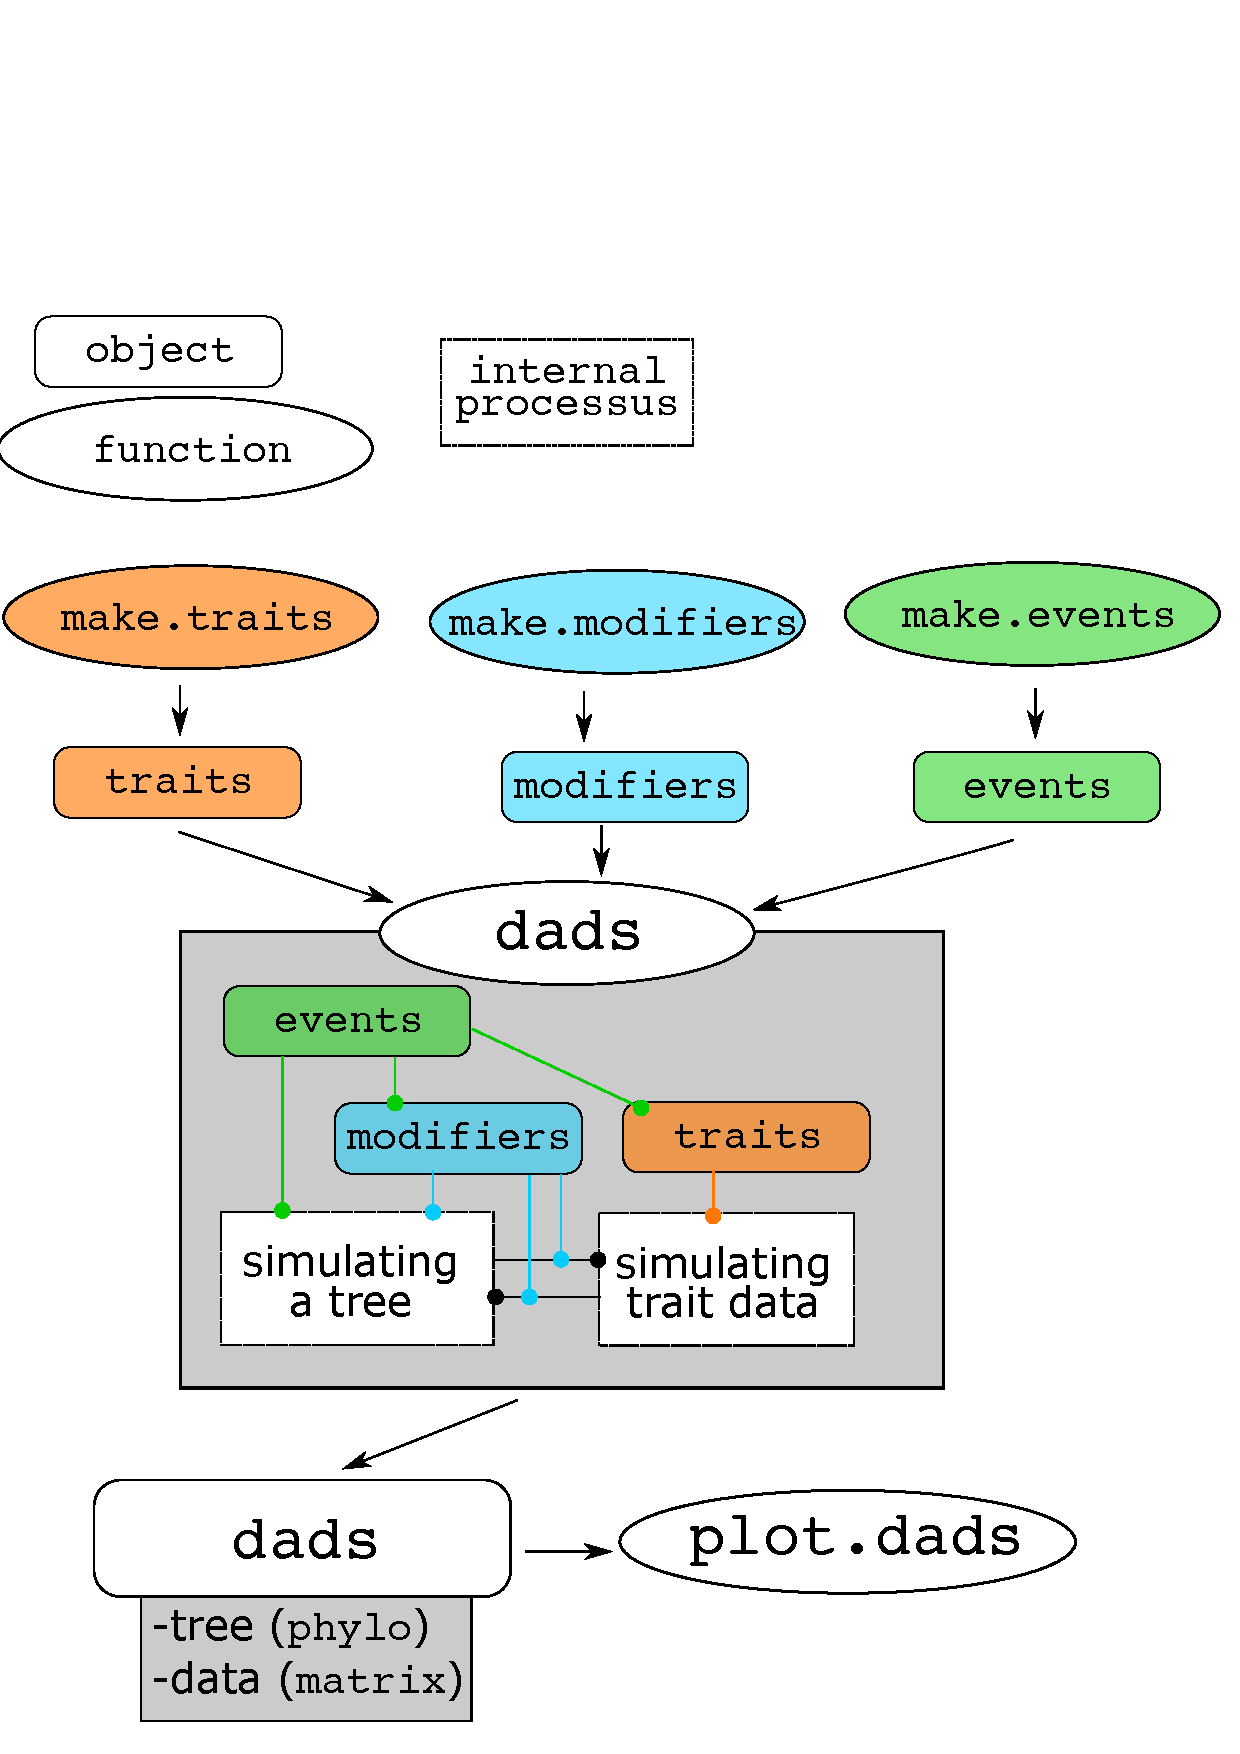
\includegraphics{dads_structure.pdf}
\caption{Schematised summary of the \texttt{dads} package architecture}
\end{figure}

\begin{verbatim}
## Loading required package: dispRity
\end{verbatim}

\hypertarget{getting-started}{%
\chapter{Getting started}\label{getting-started}}

\hypertarget{the-simplest-of-all-analysis-simulating-diversity-only}{%
\section{The simplest of all analysis: simulating diversity only}\label{the-simplest-of-all-analysis-simulating-diversity-only}}

One of the simplest things to do with the \texttt{dads} package is just to simulate a birth death tree.
For that you can use the function \texttt{dads} and specify your stopping rule.
The stopping rule simply tells the birth death process to step whenever it reaches one of these three conditions:

\begin{itemize}
\tightlist
\item
  \texttt{"max.taxa"\ \ \ =\ n} stop when \texttt{n} taxa are generated;
\item
  \texttt{"max.living"\ =\ n} stop when there is \texttt{n} co-occuring taxa of the same age (i.e. ``living'' taxa);
\item
  \texttt{"max.time"\ \ \ =\ n} stop when the simulated tree is \texttt{n} units of age old (these units are arbitrary);
\end{itemize}

For example, we might want to generate a birth-death tree with 20 taxa:

\begin{Shaded}
\begin{Highlighting}[]
\CommentTok{## Setting a stopping rule to reach a maximum of 20 taxa}
\NormalTok{my_stop_rule <-}\StringTok{ }\KeywordTok{list}\NormalTok{(}\DataTypeTok{max.taxa =} \DecValTok{20}\NormalTok{)}
\end{Highlighting}
\end{Shaded}

We can now run the simulations using:

\begin{Shaded}
\begin{Highlighting}[]
\CommentTok{## Running the birth death simulation}
\NormalTok{my_tree <-}\StringTok{ }\KeywordTok{dads}\NormalTok{(}\DataTypeTok{stop.rule =}\NormalTok{ my_stop_rule)}
\end{Highlighting}
\end{Shaded}

\begin{quote}
Note that here we could have specified more than one stopping rule, for example, we might want to run a simulation and stop it if it either reaches 10 taxa or the age 2 using \texttt{stop.rule\ =\ list(max.time\ =\ 2,\ max.taxa\ =\ 10)}. The simulation will then stop when either of these conditions are met.
\end{quote}

The resulting object is a classic \texttt{"phylo"} object that you can simply plot or visualise like so:

\begin{Shaded}
\begin{Highlighting}[]
\CommentTok{## The tree object}
\NormalTok{my_tree}
\end{Highlighting}
\end{Shaded}

\begin{verbatim}
## 
## Phylogenetic tree with 20 tips and 19 internal nodes.
## 
## Tip labels:
##   t1, t2, t3, t4, t5, t6, ...
## Node labels:
##   n1, n2, n3, n4, n5, n6, ...
## 
## Rooted; includes branch lengths.
\end{verbatim}

\begin{Shaded}
\begin{Highlighting}[]
\CommentTok{## Plotting it}
\KeywordTok{plot}\NormalTok{(my_tree)}
\end{Highlighting}
\end{Shaded}

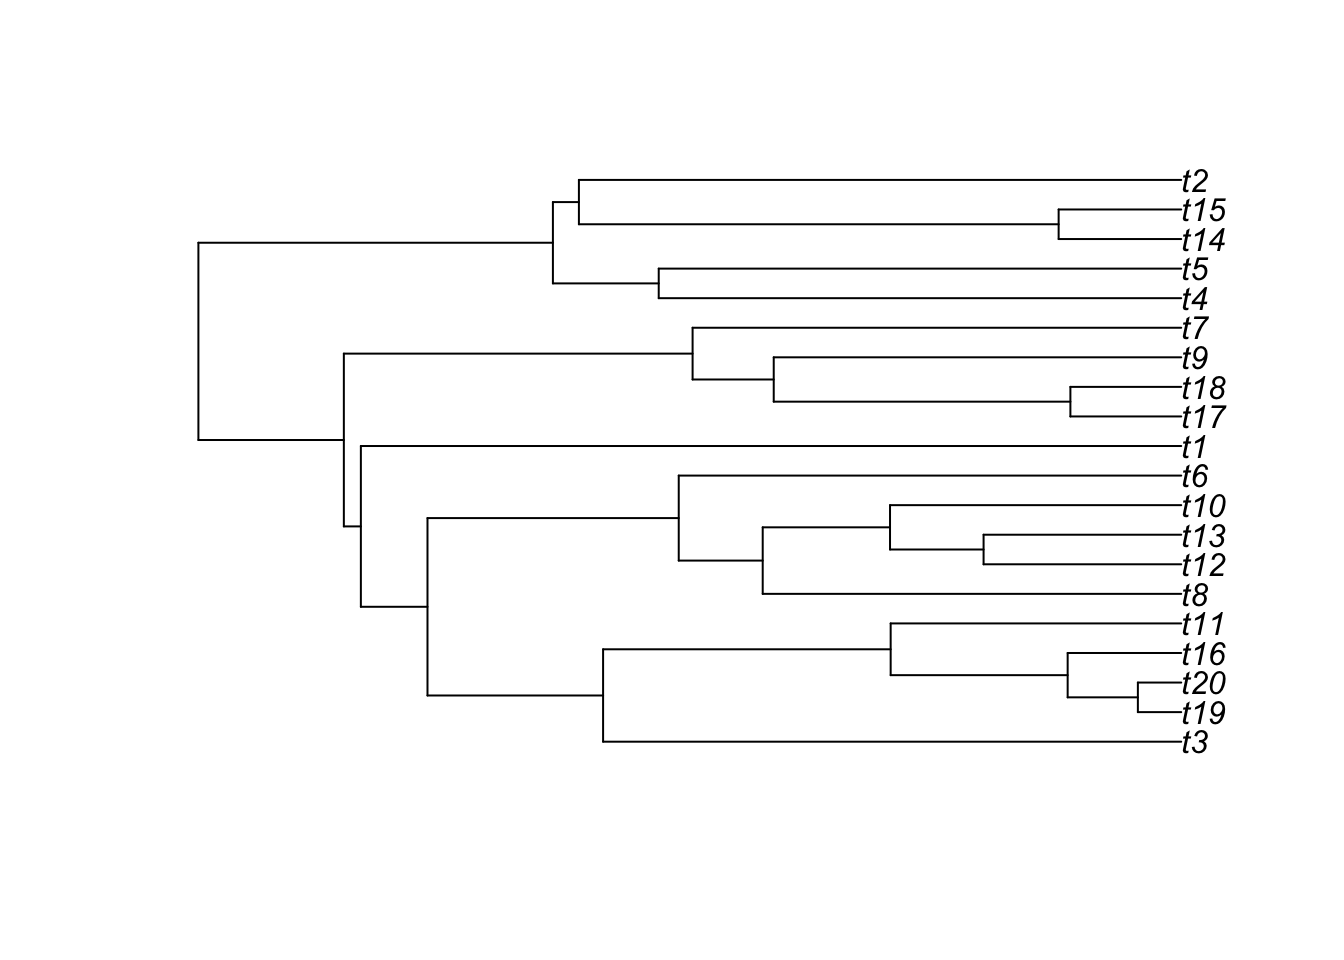
\includegraphics{dads_manual_files/figure-latex/unnamed-chunk-6-1.pdf}

\hypertarget{changing-the-birth-death-parameters}{%
\subsection{Changing the birth-death parameters}\label{changing-the-birth-death-parameters}}

People familiar with the \href{https://lukejharmon.github.io/pcm/chapter10_birthdeath/}{birth-death models} might have noticed that we did not specify two important things here: the speciation parameter (sometimes called ``lambda'' or ``birth'') and the extinction parameter (sometimes called ``mu'', ``death'' or ``background extinction'').
By default \texttt{dads} runs a pure birth model (the speciation is set to 1 and the extinction to 0).
However, you can easily change that by specifying your new birth death parameters:

\begin{Shaded}
\begin{Highlighting}[]
\CommentTok{## my birth death parameters}
\NormalTok{my_params <-}\StringTok{ }\KeywordTok{list}\NormalTok{(}\DataTypeTok{speciation =} \DecValTok{1}\NormalTok{,}
                  \DataTypeTok{extinction =} \DecValTok{1}\OperatorTok{/}\DecValTok{3}\NormalTok{)}
\end{Highlighting}
\end{Shaded}

\begin{quote}
Note that here it is not necessary to specify \texttt{extinction\ =\ 1} since this is the default option, you can always just change the parameter of interest (e.g.~changing \texttt{extinciton\ =\ 0} to \texttt{extinction\ =\ 1/3}). However, we think it's good practice to attribute both parameters specifically to avoid any confusion.
\end{quote}

You can then run the same birth death tree with extinction:

\begin{Shaded}
\begin{Highlighting}[]
\CommentTok{## Generating a birth death tree with extinctions:}
\NormalTok{my_tree <-}\StringTok{ }\KeywordTok{dads}\NormalTok{(}\DataTypeTok{bd.params =}\NormalTok{ my_params, }\DataTypeTok{stop.rule =}\NormalTok{ my_stop_rule)}
\CommentTok{## Visualising the new tree}
\KeywordTok{plot}\NormalTok{(my_tree)}
\end{Highlighting}
\end{Shaded}

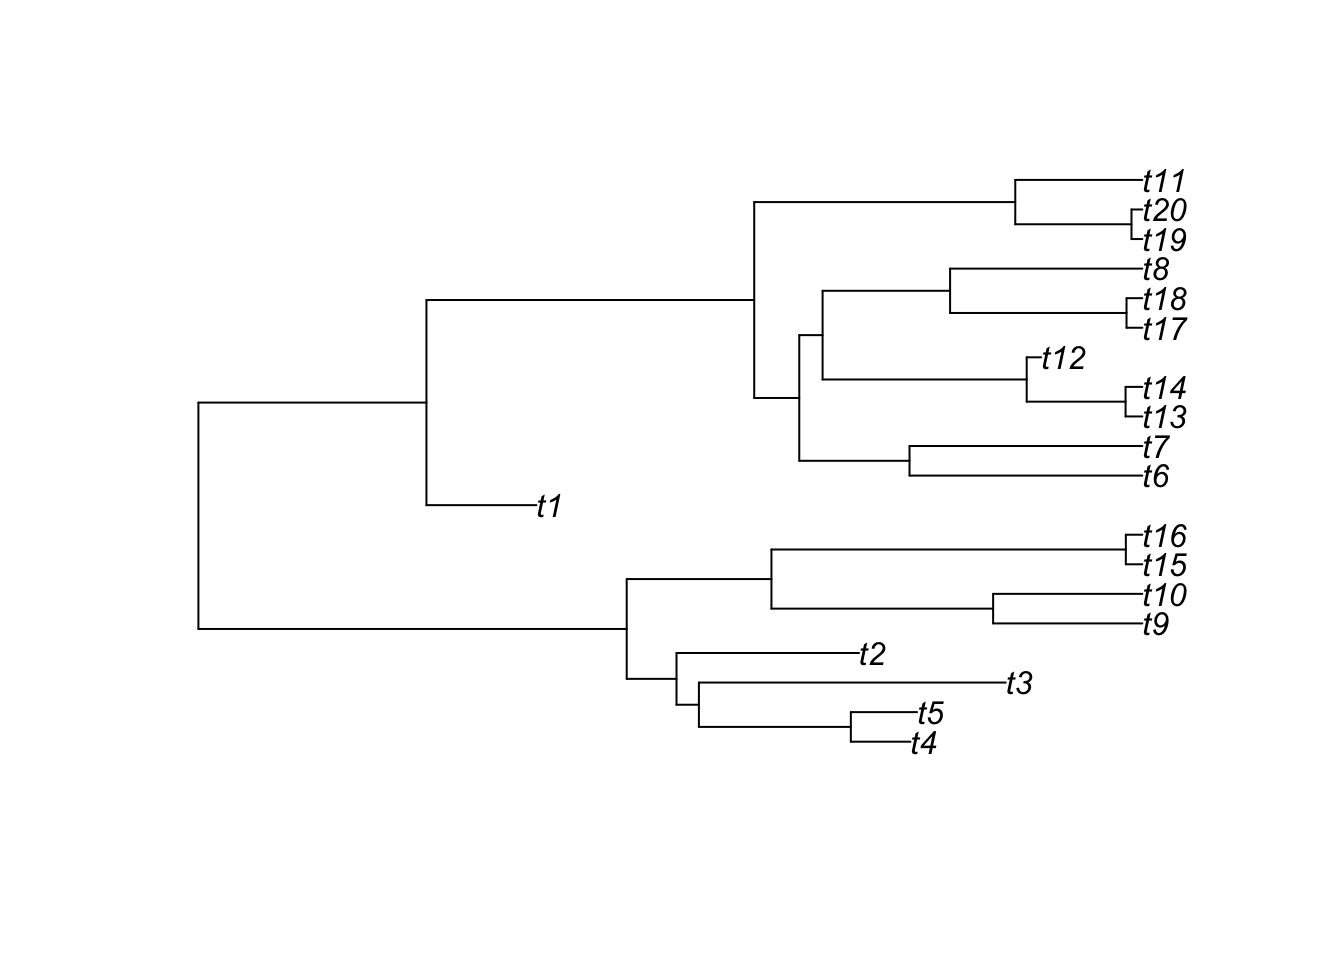
\includegraphics{dads_manual_files/figure-latex/unnamed-chunk-8-1.pdf}

\hypertarget{slightly-more-complex-simulating-disparity-and-diversity}{%
\section{Slightly more complex: simulating disparity and diversity}\label{slightly-more-complex-simulating-disparity-and-diversity}}

Chances are that you want to also simulate traits (disparity) along with your diversity (otherwise, we suggest using the \href{https://github.com/tanja819/TreeSim/}{\texttt{TreeSim}} package that provides many more birth death models).
Simulating traits is not much more complicated in \texttt{dads}: you'll simply need to create a \texttt{"traits"} object using the \texttt{make.traits} function.
These objects can have increasing complexity (see the rest of this tutorial) but we will keep it simple here.

\texttt{"traits"} objects contain one or more processes which are the ways to generate the trait.
The most common of these processes is the \href{https://en.wikipedia.org/wiki/Brownian_motion}{Brownian Motion}.
This is used by default with the \texttt{make.traits} function:

\begin{Shaded}
\begin{Highlighting}[]
\CommentTok{## Creating the traits object}
\NormalTok{my_trait <-}\StringTok{ }\KeywordTok{make.traits}\NormalTok{()}
\end{Highlighting}
\end{Shaded}

This trait object can be simply printed (to see what's in it) or plotted (to see what the process looks like in the absence of a phylogeny):

\begin{Shaded}
\begin{Highlighting}[]
\CommentTok{## Which process is in here?}
\NormalTok{my_trait}
\end{Highlighting}
\end{Shaded}

\begin{verbatim}
##  ---- dads traits object ---- 
## 1 trait for 1 process (A) with one starting value (0).
\end{verbatim}

\begin{Shaded}
\begin{Highlighting}[]
\CommentTok{## What does it look like?}
\KeywordTok{plot}\NormalTok{(my_trait)}
\end{Highlighting}
\end{Shaded}

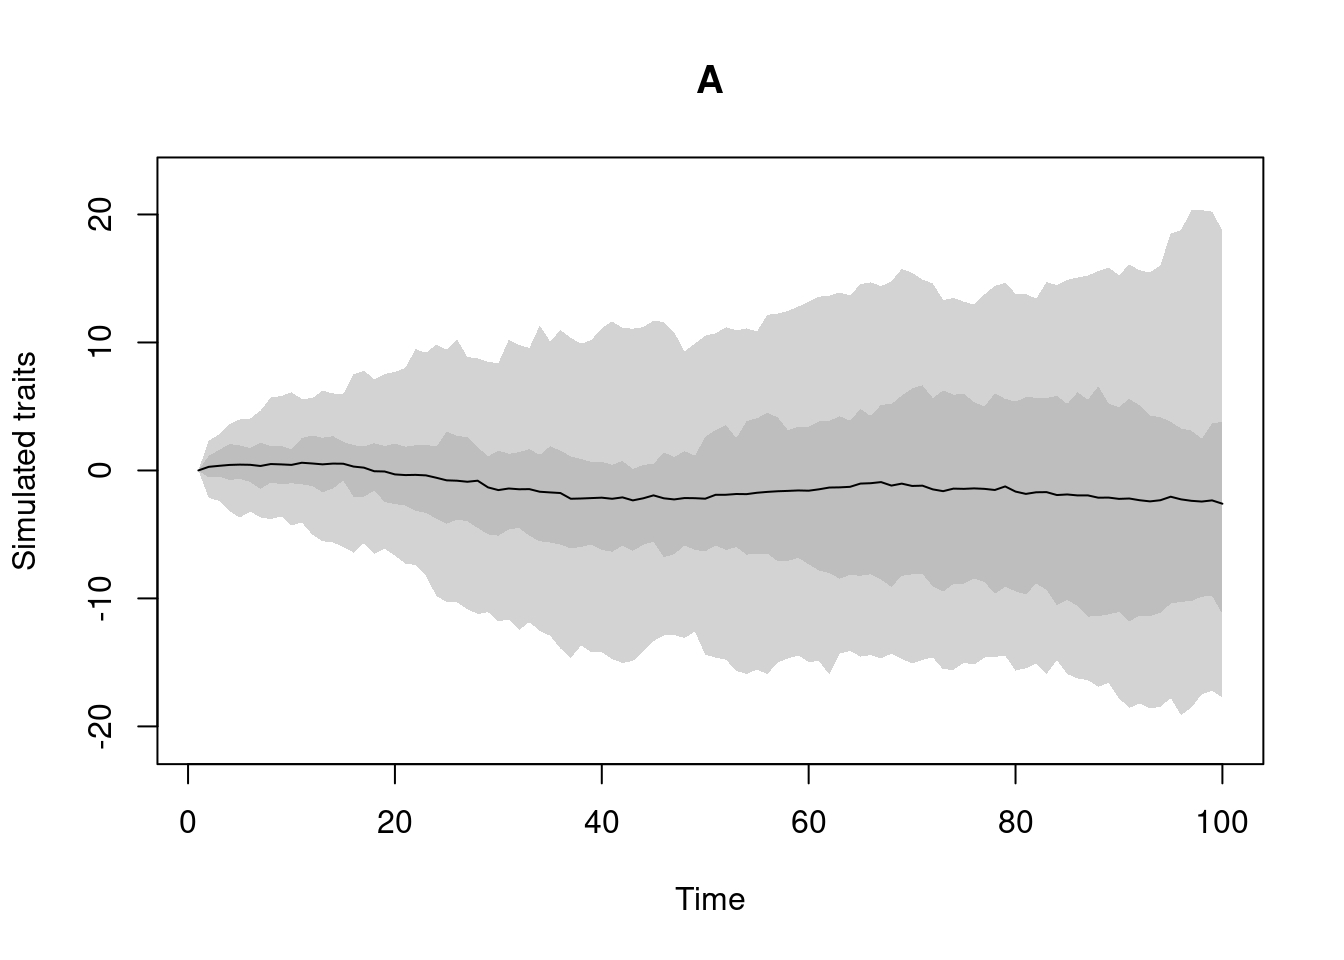
\includegraphics{dads_manual_files/figure-latex/unnamed-chunk-10-1.pdf}

By default, this trait is called ``A''.
This is not a really good name but you'll see more about specifying trait names later on.
If this is what the process should look like (theoretically) you can then add its \texttt{"traits"} object to our previous \texttt{dads} function to generate the tree and the traits:

\begin{Shaded}
\begin{Highlighting}[]
\CommentTok{## Simulate disparity and diversity}
\NormalTok{my_data <-}\StringTok{ }\KeywordTok{dads}\NormalTok{(}\DataTypeTok{bd.params =}\NormalTok{ my_params,}
                \DataTypeTok{stop.rule =}\NormalTok{ my_stop_rule,}
                \DataTypeTok{traits    =}\NormalTok{ my_trait)}
\end{Highlighting}
\end{Shaded}

Et voilà! We now have a simple disparity and diversity simulation.
We can see what's in the results by simply printing it or plotting it:

\begin{Shaded}
\begin{Highlighting}[]
\CommentTok{## What's in there}
\NormalTok{my_data}
\end{Highlighting}
\end{Shaded}

\begin{verbatim}
##  ---- dads object ---- 
## Simulated diversity data (x$tree):
## 
## Phylogenetic tree with 20 tips and 19 internal nodes.
## 
## Tip labels:
##   t1, t2, t3, t4, t5, t6, ...
## Node labels:
##   n1, n2, n3, n4, n5, n6, ...
## 
## Rooted; includes branch lengths.
## 
## Simulated disparity data (x$data):
## 1 trait for 1 process (A) with one starting value (0).
\end{verbatim}

\begin{Shaded}
\begin{Highlighting}[]
\CommentTok{## Plotting the disparity and diversity}
\KeywordTok{plot}\NormalTok{(my_data)}
\end{Highlighting}
\end{Shaded}

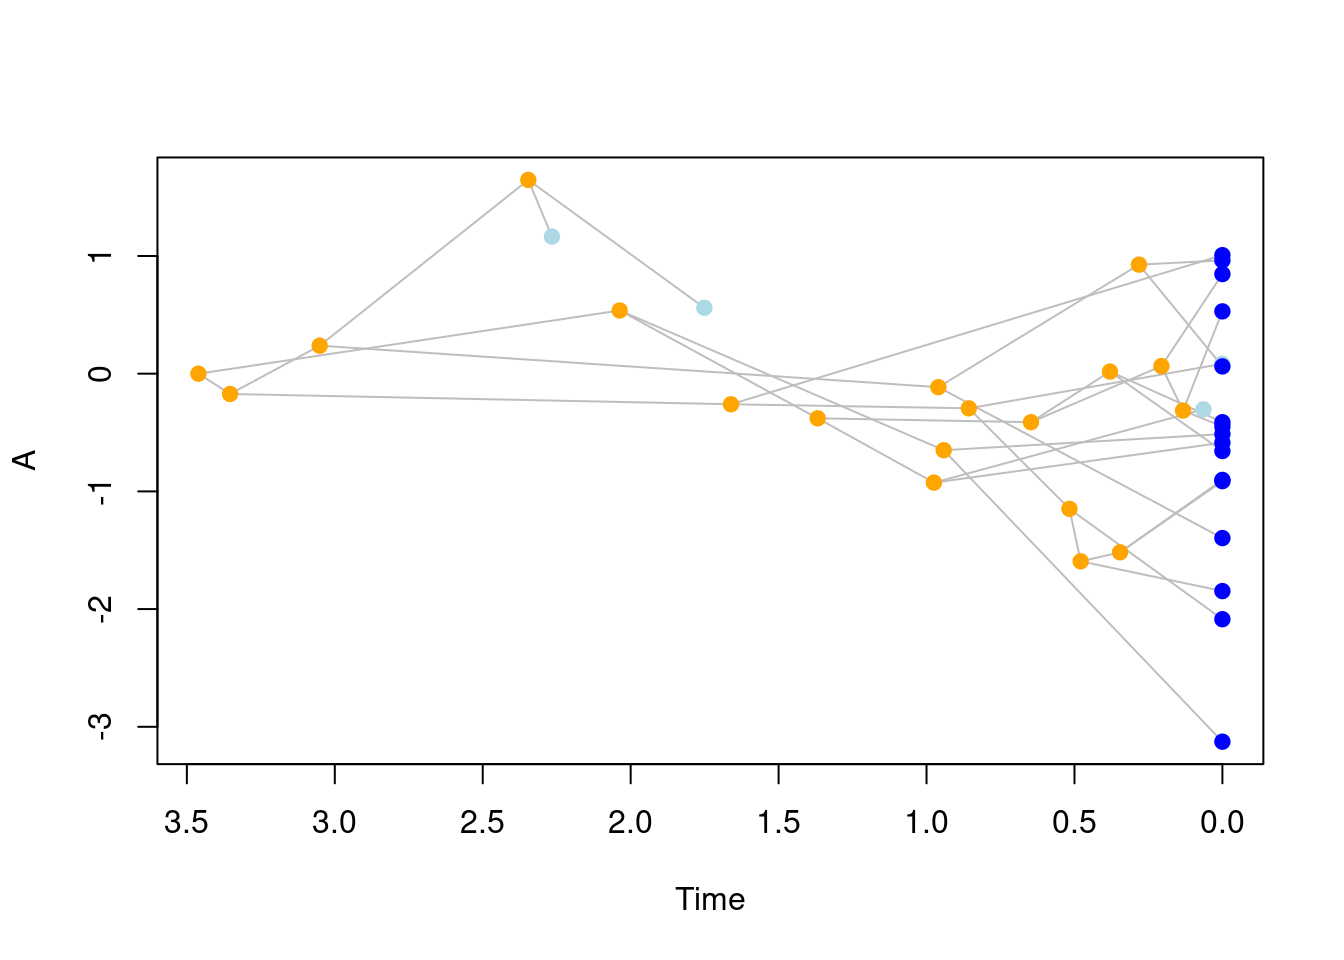
\includegraphics{dads_manual_files/figure-latex/unnamed-chunk-12-1.pdf}

You can then extract the components you need for your specific analysis like so:

\begin{Shaded}
\begin{Highlighting}[]
\CommentTok{## Extracting the tree (a "phylo" object)}
\NormalTok{the_generated_tree <-}\StringTok{ }\NormalTok{my_data}\OperatorTok{$}\NormalTok{tree}
\KeywordTok{class}\NormalTok{(the_generated_tree)}
\end{Highlighting}
\end{Shaded}

\begin{verbatim}
## [1] "phylo"
\end{verbatim}

\begin{Shaded}
\begin{Highlighting}[]
\CommentTok{## Extracting the data (a "matrix")}
\NormalTok{the_generated_data <-}\StringTok{ }\NormalTok{my_data}\OperatorTok{$}\NormalTok{data}
\KeywordTok{class}\NormalTok{(the_generated_data)}
\end{Highlighting}
\end{Shaded}

\begin{verbatim}
## [1] "matrix" "array"
\end{verbatim}

You can find much more on how to design trait objects in the \protect\hyperlink{maketraits}{\texttt{make.traits} section}.

\hypertarget{slightly-more-more-complex-simulating-linked-disparity-and-diversity}{%
\section{Slightly more more complex: simulating linked disparity and diversity}\label{slightly-more-more-complex-simulating-linked-disparity-and-diversity}}

The example above is also still pretty simple and easily done through a variety of \texttt{R} packages: here the trait and the tree are simulated at the same time but only the tree is simulating the trait (i.e.~the trait value at a tip is affected by it's ancestor and the branch length leading to it) but not the other way around (the trait value does not affect the tree).
It is possible to add this aspect using \texttt{"modifiers"} objects.
\texttt{"modifiers"} are similar to \texttt{"traits"} in that you specify what should go in there and then feed it to your simulation.

\texttt{"modifiers"} affect two key steps of the birth-death process: the calculation of the waiting time (i.e.~the component generating branch lengths) and the triggering of speciation or extinction events.
These events can be modified using some \texttt{condition} and \texttt{modify} function.
In other words, when reaching a certain condition specified by a \texttt{condition} function, the birth-death process will modify either the branch length or the speciation (or extinction) probability by applying a \texttt{modify} function.

You can use the function \texttt{make.modifiers} to design a specific \texttt{"modifiers"} object.
By default, this function generates a \texttt{"modifiers"} object that affects branch length and speciation in the following way:

\begin{itemize}
\tightlist
\item
  branch length is a randomly drawn number from an exponential distribution with a rate equal to the current number of taxa multiplied by the sum of the speciation and extinction rates.
\item
  speciation is triggered if a randomly drawn number (from a (0,1) uniform distribution) is smaller than the ratio between the speciation rate and the sum of the speciation and extinction rates. If that random number is greater, the lineage goes extinct.
\end{itemize}

Note that these are default for a birth death tree and were actually already applied in the examples before (without specifying a modifier):

\begin{Shaded}
\begin{Highlighting}[]
\CommentTok{## Make a default modifiers}
\NormalTok{default_modifiers <-}\StringTok{ }\KeywordTok{make.modifiers}\NormalTok{()}
\CommentTok{## What's in it?}
\NormalTok{default_modifiers}
\end{Highlighting}
\end{Shaded}

\begin{verbatim}
##  ---- dads modifiers object ---- 
## No modifiers applied to the branch length and speciation processes (default).
\end{verbatim}

This will not do much to our simulations compared to the previous trait and tree simulation but we can provide our modifiers object to the \texttt{dads} function:

\begin{Shaded}
\begin{Highlighting}[]
\KeywordTok{set.seed}\NormalTok{(}\DecValTok{1}\NormalTok{)}
\CommentTok{## Setting the simulation parameters}
\NormalTok{extinction_}\DecValTok{02}\NormalTok{ <-}\StringTok{ }\KeywordTok{list}\NormalTok{(}\DataTypeTok{extinction =} \FloatTok{0.4}\NormalTok{)}
\NormalTok{living_}\DecValTok{20}\NormalTok{     <-}\StringTok{ }\KeywordTok{list}\NormalTok{(}\DataTypeTok{max.living =} \DecValTok{20}\NormalTok{)}
\NormalTok{BM_trait      <-}\StringTok{ }\KeywordTok{make.traits}\NormalTok{()}
\KeywordTok{set.seed}\NormalTok{(}\DecValTok{4242}\NormalTok{)}
\CommentTok{## Simulate disparity and diversity}
\NormalTok{default_data <-}\StringTok{ }\KeywordTok{dads}\NormalTok{(}\DataTypeTok{bd.params =}\NormalTok{ extinction_}\DecValTok{02}\NormalTok{,}
                     \DataTypeTok{stop.rule =}\NormalTok{ living_}\DecValTok{20}\NormalTok{,}
                     \DataTypeTok{traits    =}\NormalTok{ BM_trait,}
                     \DataTypeTok{modifiers =}\NormalTok{ default_modifiers)}
\NormalTok{default_data}
\end{Highlighting}
\end{Shaded}

\begin{verbatim}
##  ---- dads object ---- 
## Birth death process with modifiers:
## No modifiers applied to the branch length and speciation processes (default).
## 
## Simulated diversity data (x$tree):
## 
## Phylogenetic tree with 45 tips and 44 internal nodes.
## 
## Tip labels:
##   t1, t2, t3, t4, t5, t6, ...
## Node labels:
##   n1, n2, n3, n4, n5, n6, ...
## 
## Rooted; includes branch lengths.
## 
## Simulated disparity data (x$data):
## 1 trait for 1 process (A) with one starting value (0).
\end{verbatim}

Note however that the printing information is now updated to state that you've add a modifier (even though it's a default one).

For more interesting simulations however, you can provide modifiers that actually modify the birth death process.
We can create one for example that makes species go extinct if their ancestor have a negative trait value.
For that we need to create a modifiers object that modifies the \texttt{speciation} process with a specific condition and a specific modification when that condition is met.
First we are going to create the modification function.
This function must intake the argument \texttt{x} and, in our case, return a logical value: \texttt{TRUE} is for speciate and \texttt{FALSE} is for go extinct.
We want this \texttt{modify} function to always return \texttt{FALSE} (go extinct) since it will be triggered by \texttt{condition} (we will see that in a minute).

\begin{Shaded}
\begin{Highlighting}[]
\CommentTok{## Going extinct}
\NormalTok{staying.alive <-}\StringTok{ }\ControlFlowTok{function}\NormalTok{(x) }\KeywordTok{return}\NormalTok{(}\OtherTok{TRUE}\NormalTok{)}
\end{Highlighting}
\end{Shaded}

Now we want this function to only trigger when an ancestor has a negative trait value.
We can do that by specifying our \texttt{condition} function (when the ancestor is trait is negative) apply our modification (here the \texttt{staying.alive} function).
For that we can use the \texttt{parent.traits} utility function that is optimised for accessing traits in the birth death process (but you can of course write your own).
This function intakes the \texttt{trait.values} and \texttt{parent.lineage} arguments, two arguments that you can leave named as they are to facilitate \texttt{dads}s understanding of what you which to asses:

\begin{Shaded}
\begin{Highlighting}[]
\CommentTok{## Triggering a modification only if the ancestor trait is negative}
\NormalTok{negative.ancestor <-}\StringTok{ }\ControlFlowTok{function}\NormalTok{(trait.values, parent.lineage) \{}
    \KeywordTok{return}\NormalTok{(}\KeywordTok{all}\NormalTok{(}\KeywordTok{parent.traits}\NormalTok{(trait.values, parent.lineage) }\OperatorTok{<}\StringTok{ }\DecValTok{0}\NormalTok{))}
\NormalTok{\}}
\end{Highlighting}
\end{Shaded}

Note that we use the function \texttt{all} here to evaluate all traits (if the data is multidimensional).
We can then provide these two functions (the condition \texttt{negative.ancestor} and how to modify the speciation event when this condition is met \texttt{staying.alive}).
If you are an advances \texttt{dads} user, you can design your own \texttt{speciation} function but if you just want to use a normal \texttt{speciation} function, you can use the default one from \texttt{dads} called\ldots{} \texttt{speciation}.

\begin{Shaded}
\begin{Highlighting}[]
\CommentTok{## Making a modifier for species to go extinct if}
\CommentTok{## their ancestor's trait value is (or are) negative}
\NormalTok{negatives_extinct <-}\StringTok{ }\KeywordTok{make.modifiers}\NormalTok{(}
                        \CommentTok{## The speciation function (default)}
                        \DataTypeTok{speciation =}\NormalTok{ speciation,}
                        \CommentTok{## What to modify}
                        \DataTypeTok{modify     =}\NormalTok{ staying.alive,}
                        \CommentTok{## When to modify it}
                        \DataTypeTok{condition  =}\NormalTok{ negative.ancestor)}
\CommentTok{## What's in it?}
\NormalTok{negatives_extinct}
\end{Highlighting}
\end{Shaded}

\begin{verbatim}
##  ---- dads modifiers object ---- 
## Default branch length process.
## Speciation process is set to speciation with a condition (negative.ancestor) and a modifier (staying.alive).
\end{verbatim}

Note that the \texttt{make.modifiers} function tests whether the input is compatible with \texttt{dads} by default so unless you have an error message, your \texttt{modifiers} will work!
We can now simulate our tree and traits with our modifier: species will go extinct if their ancestor have a negative trait value:

\begin{Shaded}
\begin{Highlighting}[]
\KeywordTok{set.seed}\NormalTok{(}\DecValTok{4242}\NormalTok{)}
\CommentTok{## Simulate disparity and diversity}
\NormalTok{biased_data <-}\StringTok{ }\KeywordTok{dads}\NormalTok{(}\DataTypeTok{bd.params =}\NormalTok{ extinction_}\DecValTok{02}\NormalTok{,}
                    \DataTypeTok{stop.rule =}\NormalTok{ living_}\DecValTok{20}\NormalTok{,}
                    \DataTypeTok{traits    =}\NormalTok{ BM_trait,}
                    \DataTypeTok{modifiers =}\NormalTok{ negatives_extinct)}
\NormalTok{biased_data}
\end{Highlighting}
\end{Shaded}

\begin{verbatim}
##  ---- dads object ---- 
## Birth death process with modifiers:
## Default branch length process.
## Speciation process is set to speciation with a condition (negative.ancestor) and a modifier (staying.alive).
## 
## Simulated diversity data (x$tree):
## 
## Phylogenetic tree with 38 tips and 37 internal nodes.
## 
## Tip labels:
##   t1, t2, t3, t4, t5, t6, ...
## Node labels:
##   n1, n2, n3, n4, n5, n6, ...
## 
## Rooted; includes branch lengths.
## 
## Simulated disparity data (x$data):
## 1 trait for 1 process (A) with one starting value (0).
\end{verbatim}

We can now compare the two trees and their trait values.
Note that we've used the same starting seed for both trees so the only thing differing between them is the modifier!
Also, although species

\begin{Shaded}
\begin{Highlighting}[]
\KeywordTok{par}\NormalTok{(}\DataTypeTok{mfrow =} \KeywordTok{c}\NormalTok{(}\DecValTok{1}\NormalTok{,}\DecValTok{2}\NormalTok{))}
\KeywordTok{plot}\NormalTok{(default_data, }\DataTypeTok{main =} \StringTok{"default results"}\NormalTok{)}
\KeywordTok{plot}\NormalTok{(biased_data, }\DataTypeTok{main =} \StringTok{"results with the modifier"}\NormalTok{)}
\end{Highlighting}
\end{Shaded}

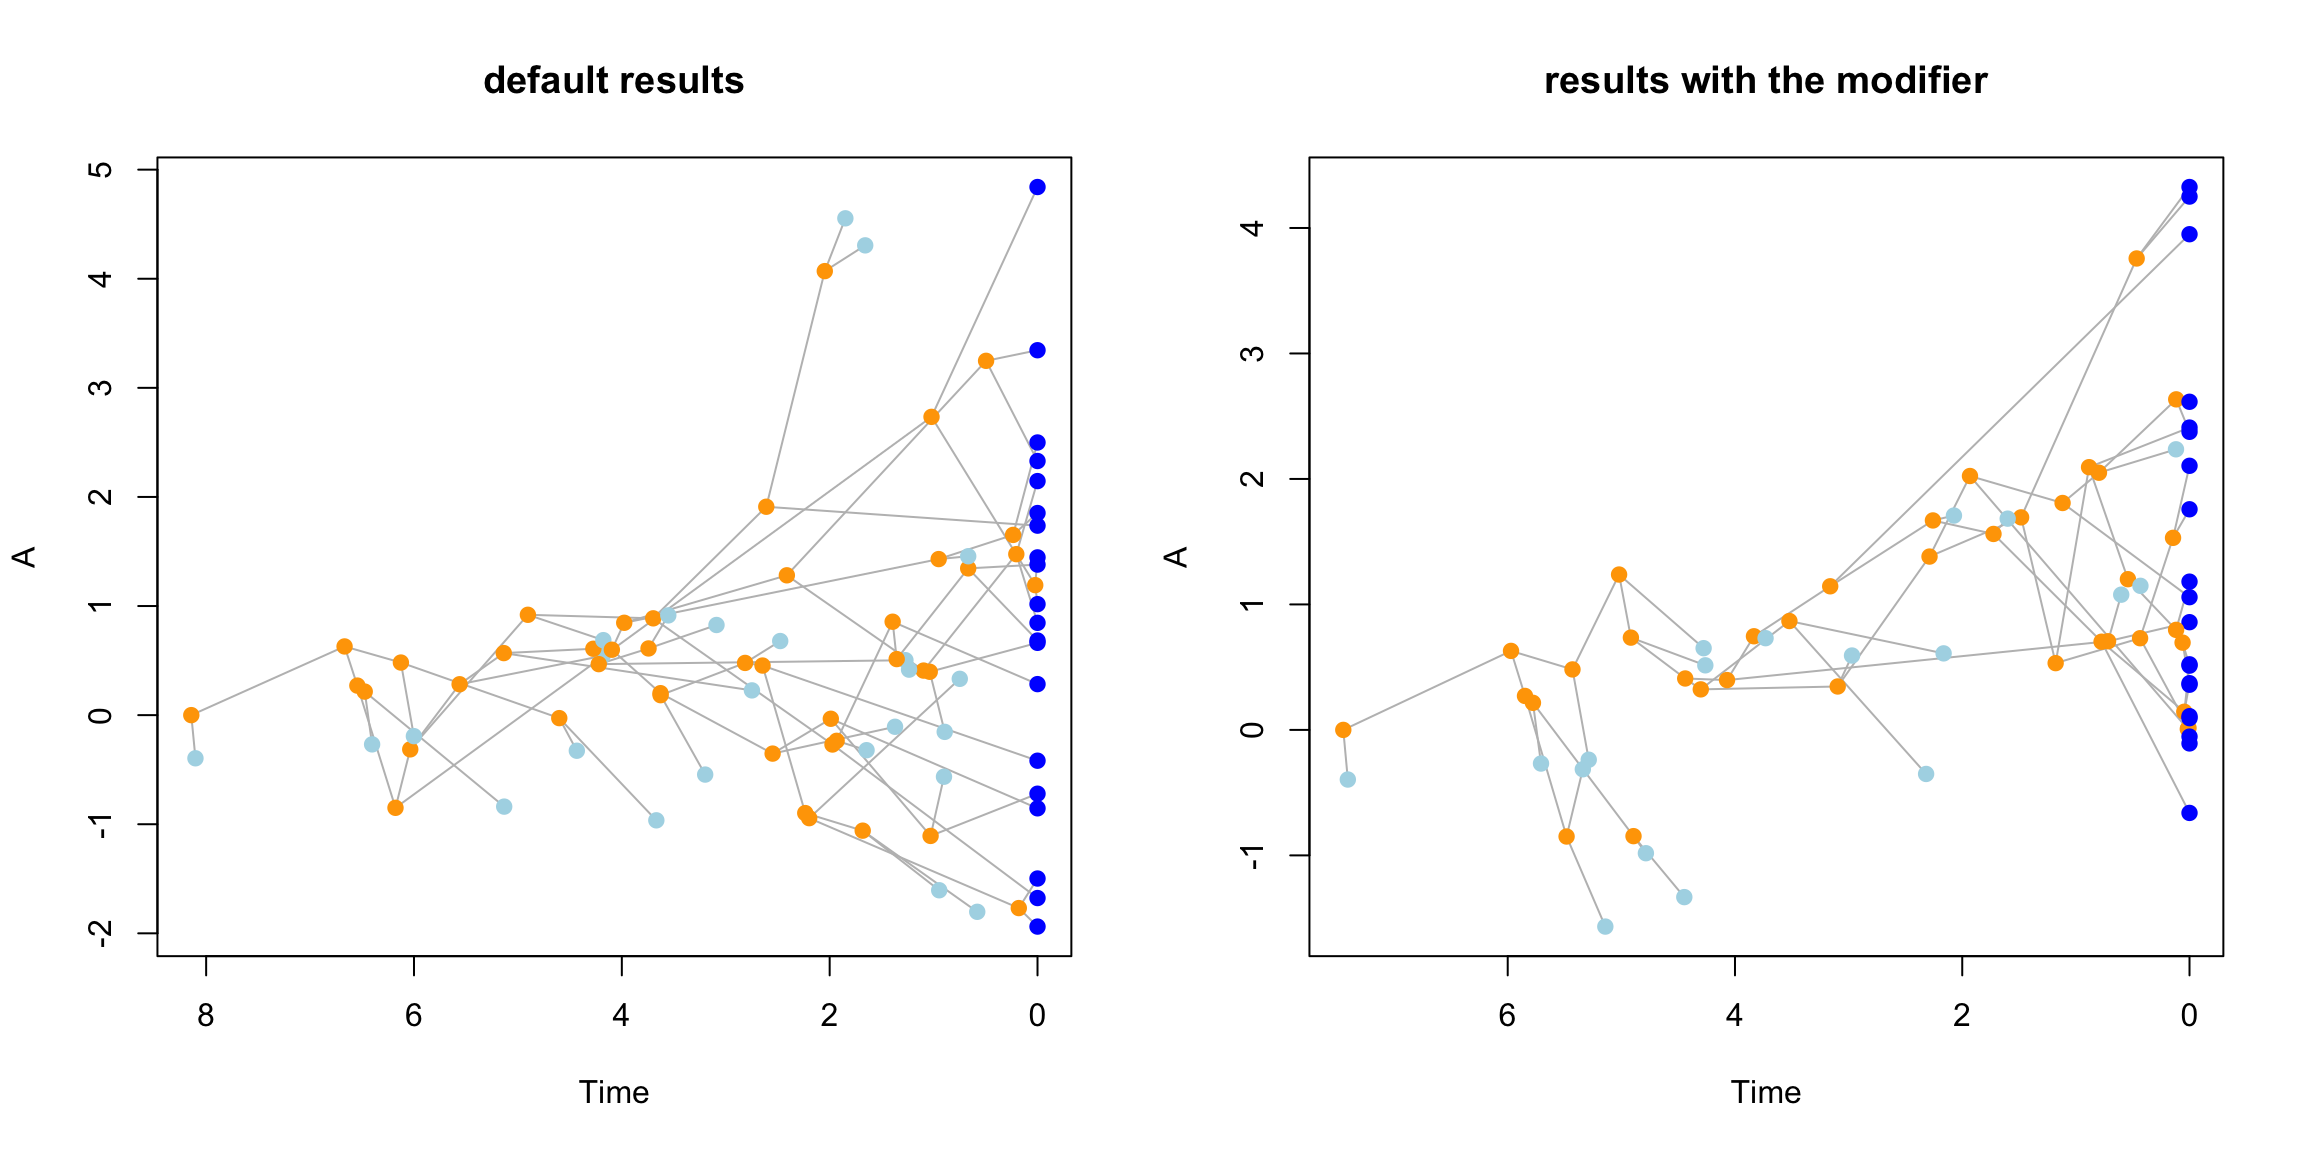
\includegraphics{dads_manual_files/figure-latex/unnamed-chunk-20-1.pdf}

You can find much more how to design modifiers in the \protect\hyperlink{makemodifiers}{\texttt{make.modifiers} section}.

\hypertarget{maketraits}{%
\chapter{\texorpdfstring{Making trait processes with \texttt{make.traits()}}{Making trait processes with make.traits()}}\label{maketraits}}

\hypertarget{the-process-process}{%
\section{\texorpdfstring{The process (\texttt{process})}{The process (process)}}\label{the-process-process}}

The function \texttt{make.traits} allows you to design the process of a trait or a set of traits.
Here, the process of a trait designates the rules to generate the trait through time while simulating a phylogeny.
This process can depend on the previous state in the tree (i.e.~the trait of the ancestor) and the branch length to the descendant.
One classic example is the \href{https://en.wikipedia.org/wiki/Brownian_motion}{Brownian motion process (or Weiner process)}.
Note that it \emph{can} depend on both the ancestor and the branch length but does \emph{not necessary needs} (i.e.~the process can be only based on the previous state or only on branch length or on neither).

Trait processes in \texttt{dads} are functions that must always intake the following arguments by default.

\begin{itemize}
\tightlist
\item
  \texttt{x0}: the previous trait value(s)
\item
  \texttt{edge.length}: the branch length value
\item
  \texttt{...}: a placeholder for any extra arguments
\end{itemize}

For example, the following function would be a valid process (though not dependent on either the previous state nor the branch length):

\begin{Shaded}
\begin{Highlighting}[]
\CommentTok{## A valid (but useless) process}
\NormalTok{valid.process <-}\StringTok{ }\ControlFlowTok{function}\NormalTok{(x0, }\DataTypeTok{egde.length =} \DecValTok{1}\NormalTok{, ...) \{}
    \KeywordTok{return}\NormalTok{(}\DecValTok{42}\NormalTok{)}
\NormalTok{\}}
\end{Highlighting}
\end{Shaded}

\begin{quote}
Note that the argument \texttt{edge.length} is set to \texttt{1} by default. In general we highly recommend to set all arguments but \texttt{x0} to a default value (this really helps the speeding up the \texttt{dads} function).
\end{quote}

On the other hand, the following process (a unidimensional Brownian motion) is incorrect (it's missing \texttt{edge.length} and \texttt{...}):

\begin{Shaded}
\begin{Highlighting}[]
\CommentTok{## A wrongly formated process}
\NormalTok{invalid.process <-}\StringTok{ }\ControlFlowTok{function}\NormalTok{(x0) \{}
    \KeywordTok{return}\NormalTok{(}\KeywordTok{rnorm}\NormalTok{(}\DecValTok{1}\NormalTok{, }\DataTypeTok{mean =}\NormalTok{ x0))}
\NormalTok{\}}
\end{Highlighting}
\end{Shaded}

The \texttt{dads} package proposes inbuilt processes, namely a multidimensional Brownian motion (\texttt{BM.process}) or a a multidimensional Ornstein-Uhlenbeck process (\texttt{OU.process}).
You can find the list of implemented process by looking at the \texttt{?trait.process} manual page in \texttt{R}.

Once a process is chosen, you can feed it to the \texttt{make.traits} function:

\begin{Shaded}
\begin{Highlighting}[]
\CommentTok{## Creating a trait object}
\NormalTok{my_trait_object <-}\StringTok{ }\KeywordTok{make.traits}\NormalTok{(}\DataTypeTok{process =}\NormalTok{ BM.process)}
\end{Highlighting}
\end{Shaded}

This creates \texttt{"dads"} \texttt{"traits"} objects that you can print, and visualise using the \texttt{plot} function:

\begin{Shaded}
\begin{Highlighting}[]
\CommentTok{## The class of the object}
\KeywordTok{class}\NormalTok{(my_trait_object)}
\end{Highlighting}
\end{Shaded}

\begin{verbatim}
## [1] "dads"   "traits"
\end{verbatim}

\begin{Shaded}
\begin{Highlighting}[]
\CommentTok{## What's in it?}
\NormalTok{my_trait_object}
\end{Highlighting}
\end{Shaded}

\begin{verbatim}
##  ---- dads traits object ---- 
## 1 trait for 1 process (A) with one starting value (0).
\end{verbatim}

\begin{Shaded}
\begin{Highlighting}[]
\CommentTok{## What does the process looks like}
\KeywordTok{plot}\NormalTok{(my_trait_object)}
\end{Highlighting}
\end{Shaded}

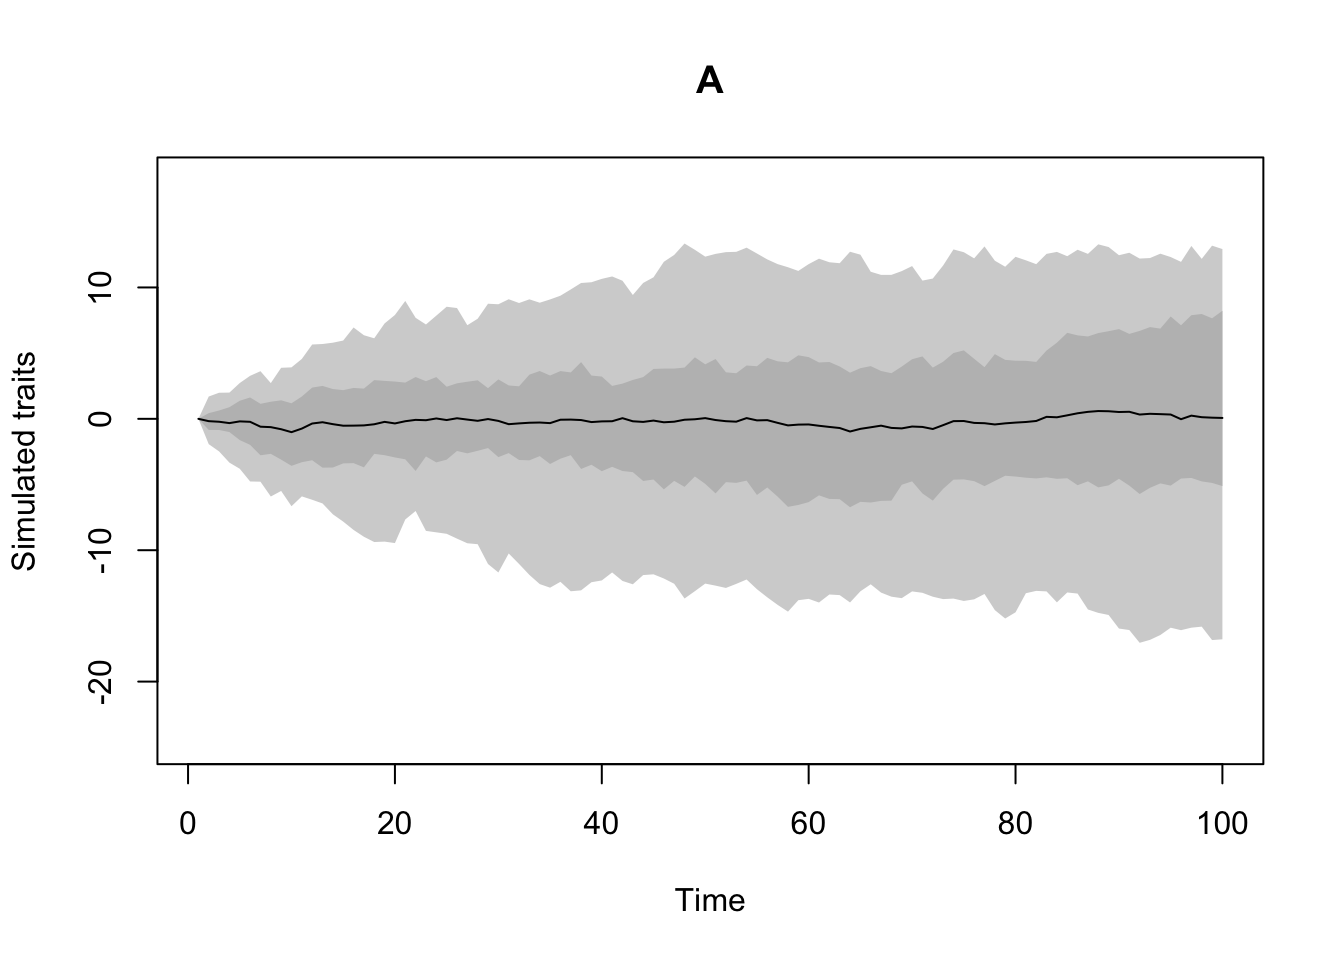
\includegraphics{dads_manual_files/figure-latex/unnamed-chunk-25-1.pdf}

Note that you can see the multiple options for plotting the trait process by looking at \texttt{?plot.dads} manual. Furthermore, you can look at what's actually in the object using:

\begin{Shaded}
\begin{Highlighting}[]
\CommentTok{## What's actually in that object?}
\KeywordTok{print.dads}\NormalTok{(my_trait_object, }\DataTypeTok{all =} \OtherTok{TRUE}\NormalTok{)}
\end{Highlighting}
\end{Shaded}

\begin{verbatim}
## $A
## $A$process
## function (x0, edge.length = 1, Sigma = diag(length(x0)), ...) 
## {
##     return(t(MASS::mvrnorm(n = 1, mu = x0, Sigma = Sigma * edge.length, 
##         ...)))
## }
## <bytecode: 0x7fd7168d5b80>
## <environment: namespace:dads>
## 
## $A$start
## [1] 0
## 
## $A$trait_id
## [1] 1
\end{verbatim}

As traits can get more and more complex, the automatic printing of its summary allows for a easier display of what's in the traits object.

Note that it is possible to make \texttt{"traits"} objects with multiple processes (that can be the same):

\begin{Shaded}
\begin{Highlighting}[]
\CommentTok{## 4 traits: two BM, one OU and one normal non process}
\NormalTok{four_traits <-}\StringTok{ }\KeywordTok{make.traits}\NormalTok{(}\DataTypeTok{process =} \KeywordTok{c}\NormalTok{(BM.process,}
\NormalTok{                                       BM.process,}
\NormalTok{                                       OU.process,}
\NormalTok{                                       no.process))}
\NormalTok{four_traits}
\end{Highlighting}
\end{Shaded}

\begin{verbatim}
##  ---- dads traits object ---- 
## 4 traits for 4 processes (A, B, C, D) with one starting value (0).
\end{verbatim}

You can visualise them individually using the \texttt{trait} argument in \texttt{plot.dads}:

\begin{Shaded}
\begin{Highlighting}[]
\CommentTok{## Plot options (4 plots in one window)}
\KeywordTok{par}\NormalTok{(}\DataTypeTok{mfrow =} \KeywordTok{c}\NormalTok{(}\DecValTok{2}\NormalTok{,}\DecValTok{2}\NormalTok{))}
\KeywordTok{plot}\NormalTok{(four_traits, }\DataTypeTok{trait =} \DecValTok{1}\NormalTok{)}
\KeywordTok{plot}\NormalTok{(four_traits, }\DataTypeTok{trait =} \DecValTok{2}\NormalTok{)}
\KeywordTok{plot}\NormalTok{(four_traits, }\DataTypeTok{trait =} \DecValTok{3}\NormalTok{)}
\KeywordTok{plot}\NormalTok{(four_traits, }\DataTypeTok{trait =} \DecValTok{4}\NormalTok{)}
\end{Highlighting}
\end{Shaded}

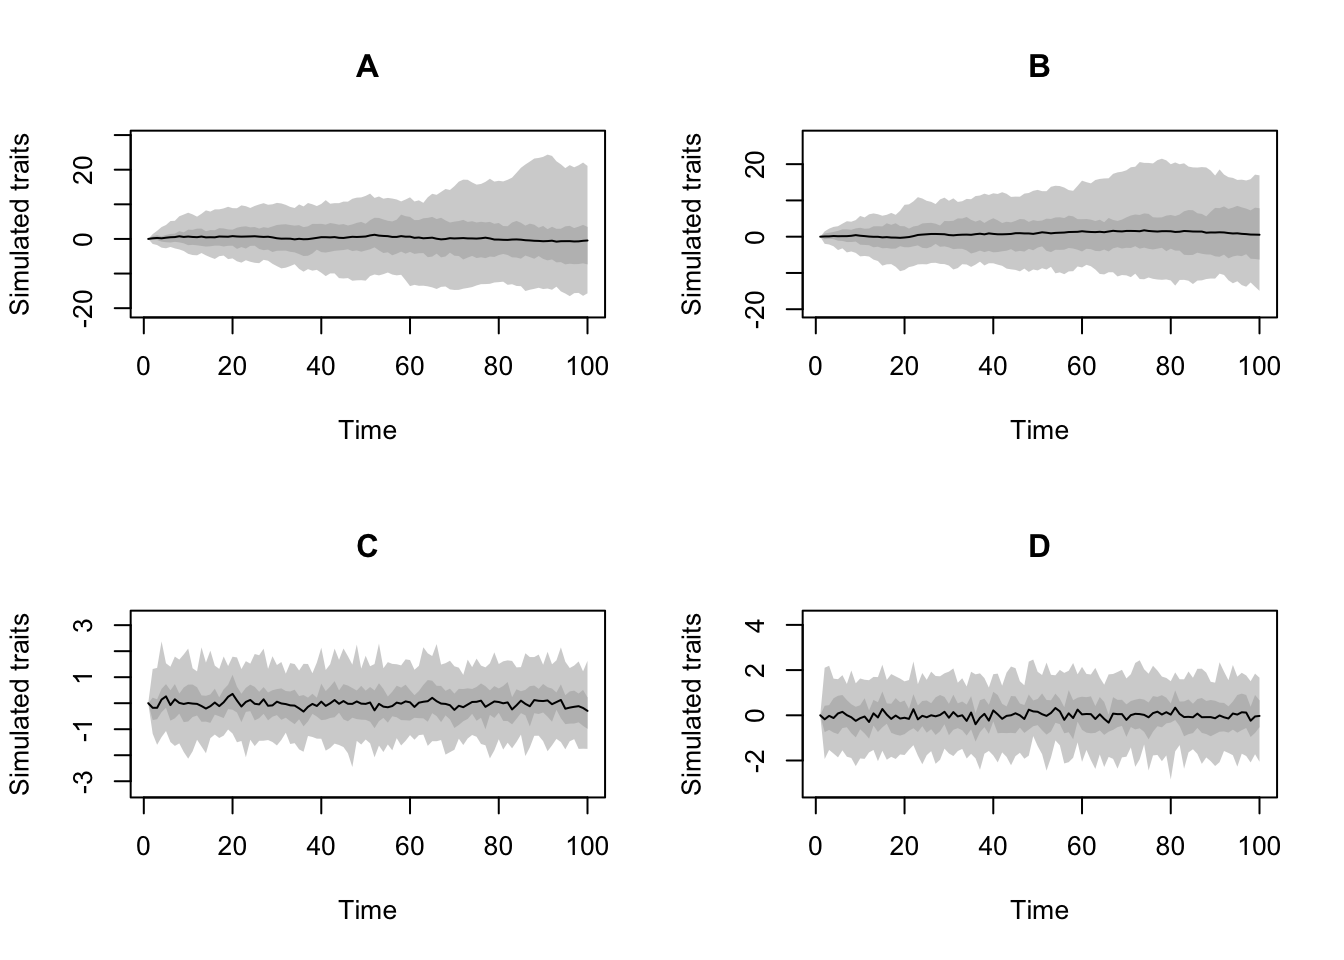
\includegraphics{dads_manual_files/figure-latex/unnamed-chunk-28-1.pdf}

\hypertarget{the-number-of-traits-n-and-the-starting-values-start}{%
\section{\texorpdfstring{The number of traits \texttt{n} and the starting values \texttt{start}}{The number of traits n and the starting values start}}\label{the-number-of-traits-n-and-the-starting-values-start}}

Two further important arguments are \texttt{n} the number of traits per process and \texttt{start} the starting values for all traits.
By default they are set to \texttt{n\ =\ 1} and \texttt{start\ =\ 0}.
This means that \texttt{make.traits} will assume that your processes are always unidimensional by default and that they always start with the value \texttt{0}.
It is however possible to change these values.

For example you can use the following to create a three dimensional Brownian motion with each dimensions starting with the value \texttt{1}:

\begin{Shaded}
\begin{Highlighting}[]
\CommentTok{## Multidimensional Brownian motion}
\KeywordTok{make.traits}\NormalTok{(BM.process, }\DataTypeTok{n =} \DecValTok{3}\NormalTok{, }\DataTypeTok{start =} \DecValTok{1}\NormalTok{)}
\end{Highlighting}
\end{Shaded}

\begin{verbatim}
##  ---- dads traits object ---- 
## 3 traits for 1 process (A:3) with one starting value (1).
\end{verbatim}

Or the following with each dimensions starting with different values (respectively \texttt{1}, \texttt{2} and \texttt{3}):

\begin{Shaded}
\begin{Highlighting}[]
\CommentTok{## Multidimensional Brownian motion}
\KeywordTok{make.traits}\NormalTok{(BM.process, }\DataTypeTok{n =} \DecValTok{3}\NormalTok{, }\DataTypeTok{start =} \KeywordTok{c}\NormalTok{(}\DecValTok{1}\NormalTok{,}\DecValTok{2}\NormalTok{,}\DecValTok{3}\NormalTok{))}
\end{Highlighting}
\end{Shaded}

\begin{verbatim}
##  ---- dads traits object ---- 
## 3 traits for 1 process (A:3) with different starting values (1,2,3).
\end{verbatim}

Note that the number of traits are distributed per processes.
If the traits contains multiple process, the number of traits are distributed per processes:

\begin{Shaded}
\begin{Highlighting}[]
\CommentTok{## two 3D processes (BM and OU)}
\KeywordTok{make.traits}\NormalTok{(}\KeywordTok{c}\NormalTok{(BM.process, OU.process), }\DataTypeTok{n =} \DecValTok{3}\NormalTok{)}
\end{Highlighting}
\end{Shaded}

\begin{verbatim}
##  ---- dads traits object ---- 
## 6 traits for 2 processes (A:3, B:3) with one starting value (0).
\end{verbatim}

\begin{Shaded}
\begin{Highlighting}[]
\CommentTok{## one 1D processes (BM) and one 4D process (OU)}
\KeywordTok{make.traits}\NormalTok{(}\KeywordTok{c}\NormalTok{(BM.process, OU.process), }\DataTypeTok{n =} \KeywordTok{c}\NormalTok{(}\DecValTok{1}\NormalTok{, }\DecValTok{4}\NormalTok{))}
\end{Highlighting}
\end{Shaded}

\begin{verbatim}
##  ---- dads traits object ---- 
## 5 traits for 2 processes (A:1, B:4) with one starting value (0).
\end{verbatim}

And starting values are distributed for all the traits or for the traits one by one:

\begin{Shaded}
\begin{Highlighting}[]
\CommentTok{## two 3D processes (BM and OU) starting with 1}
\KeywordTok{make.traits}\NormalTok{(}\KeywordTok{c}\NormalTok{(BM.process, OU.process), }\DataTypeTok{n =} \DecValTok{3}\NormalTok{, }\DataTypeTok{start =} \DecValTok{1}\NormalTok{)}
\end{Highlighting}
\end{Shaded}

\begin{verbatim}
##  ---- dads traits object ---- 
## 6 traits for 2 processes (A:3, B:3) with one starting value (1).
\end{verbatim}

\begin{Shaded}
\begin{Highlighting}[]
\CommentTok{## two 3D processes (BM and OU) starting with values 1 to 6}
\KeywordTok{make.traits}\NormalTok{(}\KeywordTok{c}\NormalTok{(BM.process, OU.process), }\DataTypeTok{n =} \DecValTok{3}\NormalTok{, }\DataTypeTok{start =} \DecValTok{1}\OperatorTok{:}\DecValTok{6}\NormalTok{)}
\end{Highlighting}
\end{Shaded}

\begin{verbatim}
##  ---- dads traits object ---- 
## 6 traits for 2 processes (A:3, B:3) with different starting values (1,2,3,4,5,6).
\end{verbatim}

\begin{Shaded}
\begin{Highlighting}[]
\CommentTok{## two 3D processes (BM and OU) with the two first ones starting}
\CommentTok{## with 1 and the 4 other ones with the default (0)}
\KeywordTok{make.traits}\NormalTok{(}\KeywordTok{c}\NormalTok{(BM.process, OU.process), }\DataTypeTok{n =} \DecValTok{3}\NormalTok{, }\DataTypeTok{start =} \KeywordTok{c}\NormalTok{(}\DecValTok{1}\NormalTok{,}\DecValTok{1}\NormalTok{))}
\end{Highlighting}
\end{Shaded}

\begin{verbatim}
## Warning in make.traits(c(BM.process, OU.process), n = 3, start = c(1, 1)): Only
## the first 2 starting values were supplied for a required 6 traits. The missing
## start values are set to 0.
\end{verbatim}

\begin{verbatim}
##  ---- dads traits object ---- 
## 6 traits for 2 processes (A:3, B:3) with different starting values (1,1,0,0,0,0).
\end{verbatim}

\hypertarget{extra-argument-for-the-processes-with-process.args}{%
\section{\texorpdfstring{Extra argument for the processes with \texttt{process.args}}{Extra argument for the processes with process.args}}\label{extra-argument-for-the-processes-with-process.args}}

You can also feed extra arguments to your process(es) functions. For example, the inbuilt process \texttt{no.process} (that is just a number generator not based on the previous value \texttt{x0} or the branch length) can intake a specific random number generator as a function:

\begin{Shaded}
\begin{Highlighting}[]
\CommentTok{## no process trait using the normal distribution (default)}
\KeywordTok{make.traits}\NormalTok{(no.process, }\DataTypeTok{process.args =} \KeywordTok{list}\NormalTok{(}\DataTypeTok{fun =}\NormalTok{ rnorm))}
\end{Highlighting}
\end{Shaded}

\begin{verbatim}
##  ---- dads traits object ---- 
## 1 trait for 1 process (A) with one starting value (0).
## process A uses the following extra argument: fun;
\end{verbatim}

\begin{Shaded}
\begin{Highlighting}[]
\CommentTok{## no process trait using the uniform distribution}
\CommentTok{## bounded between 1 and 100}
\KeywordTok{make.traits}\NormalTok{(no.process, }\DataTypeTok{process.args =} \KeywordTok{list}\NormalTok{(}\DataTypeTok{fun =}\NormalTok{ runif, }\DataTypeTok{min =} \DecValTok{1}\NormalTok{, }\DataTypeTok{max =} \DecValTok{100}\NormalTok{))}
\end{Highlighting}
\end{Shaded}

\begin{verbatim}
##  ---- dads traits object ---- 
## 1 trait for 1 process (A) with one starting value (0).
## process A uses the following extra arguments: fun,min,max;
\end{verbatim}

You can also add multiple extra arguments for multiple processes giving them as a list.

\begin{Shaded}
\begin{Highlighting}[]
\CommentTok{## Two traits with no process:one normal and one uniform (1,100)}
\KeywordTok{make.traits}\NormalTok{(}\DataTypeTok{process      =} \KeywordTok{c}\NormalTok{(no.process, no.process),}
            \DataTypeTok{process.args =} \KeywordTok{list}\NormalTok{(}\KeywordTok{list}\NormalTok{(}\DataTypeTok{fun =}\NormalTok{ rnorm),}
                                \KeywordTok{list}\NormalTok{(}\DataTypeTok{fun =}\NormalTok{ runif, }\DataTypeTok{min =} \DecValTok{1}\NormalTok{, }\DataTypeTok{max =} \DecValTok{100}\NormalTok{)))}
\end{Highlighting}
\end{Shaded}

\begin{verbatim}
##  ---- dads traits object ---- 
## 2 traits for 2 processes (A, B) with one starting value (0).
## process A uses the following extra argument: fun;
## process B uses the following extra arguments: fun,min,max;
\end{verbatim}

If one process do not need extra argument you must still give it and extra \texttt{NULL} process argument:

\begin{Shaded}
\begin{Highlighting}[]
\CommentTok{## Three traits with no process:}
\CommentTok{## one default, one lognormal and one uniform (1,100)}
\KeywordTok{make.traits}\NormalTok{(}\DataTypeTok{process      =} \KeywordTok{c}\NormalTok{(no.process, no.process, no.process),}
            \DataTypeTok{process.args =} \KeywordTok{list}\NormalTok{(}\CommentTok{## Extra arguments for the first process (none)}
                                \KeywordTok{list}\NormalTok{(}\OtherTok{NULL}\NormalTok{),}
                                \CommentTok{## Extra arguments for the second process}
                                \KeywordTok{list}\NormalTok{(}\DataTypeTok{fun =}\NormalTok{ rlnorm),}
                                \CommentTok{## Extra arguments for the third process}
                                \KeywordTok{list}\NormalTok{(}\DataTypeTok{fun =}\NormalTok{ runif, }\DataTypeTok{min =} \DecValTok{1}\NormalTok{, }\DataTypeTok{max =} \DecValTok{100}\NormalTok{)))}
\end{Highlighting}
\end{Shaded}

\begin{verbatim}
##  ---- dads traits object ---- 
## 3 traits for 3 processes (A, B, C) with one starting value (0).
## process B uses the following extra argument: fun;
## process C uses the following extra arguments: fun,min,max;
\end{verbatim}

\hypertarget{naming-the-traits-with-trait.names}{%
\section{\texorpdfstring{Naming the traits with \texttt{trait.names}}{Naming the traits with trait.names}}\label{naming-the-traits-with-trait.names}}

As traits become more and more complex, it can be useful to give clearer names to each process.
This is easily done using the \texttt{trait.names} argument that attributes one name per process:

\begin{Shaded}
\begin{Highlighting}[]
\CommentTok{## A simple trait with a proper name}
\NormalTok{simple_trait <-}\StringTok{ }\KeywordTok{make.traits}\NormalTok{(}\DataTypeTok{trait.names =} \StringTok{"1D Brownian Motion"}\NormalTok{)}
\NormalTok{simple_trait}
\end{Highlighting}
\end{Shaded}

\begin{verbatim}
##  ---- dads traits object ---- 
## 1 trait for 1 process (1D Brownian Motion) with one starting value (0).
\end{verbatim}

This becomes more useful if we use the complex example above:

\begin{Shaded}
\begin{Highlighting}[]
\CommentTok{## Three named traits with no process:}
\CommentTok{## one default, one lognormal and one uniform (1,100)}
\KeywordTok{make.traits}\NormalTok{(}\DataTypeTok{process      =} \KeywordTok{c}\NormalTok{(no.process, no.process, no.process),}
            \DataTypeTok{process.args =} \KeywordTok{list}\NormalTok{(}\CommentTok{## Extra arguments for the first process (none)}
                                \KeywordTok{list}\NormalTok{(}\OtherTok{NULL}\NormalTok{),}
                                \CommentTok{## Extra arguments for the second process}
                                \KeywordTok{list}\NormalTok{(}\DataTypeTok{fun =}\NormalTok{ rlnorm),}
                                \CommentTok{## Extra arguments for the third process}
                                \KeywordTok{list}\NormalTok{(}\DataTypeTok{fun =}\NormalTok{ runif, }\DataTypeTok{min =} \DecValTok{1}\NormalTok{, }\DataTypeTok{max =} \DecValTok{100}\NormalTok{)),}
            \CommentTok{## Naming each trait}
            \DataTypeTok{trait.names  =} \KeywordTok{c}\NormalTok{(}\StringTok{"Normal"}\NormalTok{, }\StringTok{"LogNormal"}\NormalTok{, }\StringTok{"Uniform(1,100)"}\NormalTok{))}
\end{Highlighting}
\end{Shaded}

\begin{verbatim}
##  ---- dads traits object ---- 
## 3 traits for 3 processes (Normal, LogNormal, Uniform(1,100)) with one starting value (0).
## process LogNormal uses the following extra argument: fun;
## process Uniform(1,100) uses the following extra arguments: fun,min,max;
\end{verbatim}

\hypertarget{combining-multiple-traits-with-add}{%
\section{\texorpdfstring{Combining multiple traits with \texttt{add}}{Combining multiple traits with add}}\label{combining-multiple-traits-with-add}}

You can also add traits to already existing trait objects using the simple \texttt{add} option.
This option just intakes a \texttt{"dads"} \texttt{"traits"} object and the additional process(es) will be added to it. For example:

\begin{Shaded}
\begin{Highlighting}[]
\CommentTok{## Creating on simple default Brownian motion}
\NormalTok{one_process <-}\StringTok{ }\KeywordTok{make.traits}\NormalTok{(}\DataTypeTok{trait.names =} \StringTok{"BM"}\NormalTok{)}

\CommentTok{## Creating a new trait (a 3D OU.process)}
\CommentTok{## and adding the previous one}
\NormalTok{two_processes <-}\StringTok{ }\KeywordTok{make.traits}\NormalTok{(OU.process, }\DataTypeTok{n =} \DecValTok{3}\NormalTok{, }\DataTypeTok{add =}\NormalTok{ one_process,}
                             \DataTypeTok{trait.names =} \StringTok{"3D OU"}\NormalTok{)}

\CommentTok{## Only one process}
\NormalTok{one_process}
\end{Highlighting}
\end{Shaded}

\begin{verbatim}
##  ---- dads traits object ---- 
## 1 trait for 1 process (BM) with one starting value (0).
\end{verbatim}

\begin{Shaded}
\begin{Highlighting}[]
\CommentTok{## The two processes}
\NormalTok{two_processes}
\end{Highlighting}
\end{Shaded}

\begin{verbatim}
##  ---- dads traits object ---- 
## 4 traits for 2 processes (BM:1, 3D OU:3) with one starting value (0).
\end{verbatim}

\hypertarget{testing-the-traits-with-test}{%
\section{\texorpdfstring{Testing the traits with \texttt{test}}{Testing the traits with test}}\label{testing-the-traits-with-test}}

This bit is more for development.
We highly suggest leaving \texttt{test\ =\ TRUE} so that \texttt{make.traits} returns an error if a process or its additional arguments (\texttt{process.args}) are not formatted correctly.
\texttt{make.traits} will error if the trait cannot be directly passed to \texttt{dads}.
However, in some specific cases (again, probably mainly for development and debugging) it could be useful to skip the tests using \texttt{test\ =\ FALSE}.

\hypertarget{templates-for-making-your-very-own-process}{%
\section{Templates for making your very own process}\label{templates-for-making-your-very-own-process}}

As detailed above, any process of your own design will work as long as it is a function that takes at least the arguments \texttt{x0} and \texttt{edge.length}.
You can be imaginative and creative when designing your own process but here are two detailed example functions for a unidimensional Brownian Motion and Ornstein-Uhlenbeck process that you can use for a start (or not).
Remember it is good practice for \texttt{dads} processes to set all the arguments but \texttt{x0} with default values (just in case).
Also, note that the functions below are not equal to the already implemented \texttt{BM.process} and \texttt{OU.process} but are rather generalised/simplified version that you can use as a template

\hypertarget{a-simple-brownian-motion-process-template}{%
\subsection{A simple Brownian Motion process template}\label{a-simple-brownian-motion-process-template}}

\begin{Shaded}
\begin{Highlighting}[]
\CommentTok{## A simple Brownian motion process}
\NormalTok{my.BM.process <-}\StringTok{ }\ControlFlowTok{function}\NormalTok{(x0, }\DataTypeTok{edge.length =} \DecValTok{1}\NormalTok{, }\DataTypeTok{sd =} \DecValTok{1}\NormalTok{, ...) \{}
    \CommentTok{## Drawing a random number from a normal distribution}
    \CommentTok{## with x0 as the and a given standard deviation}
    \CommentTok{## and depending on branch (edge) length}
\NormalTok{    result <-}\StringTok{ }\KeywordTok{rnorm}\NormalTok{(}\DataTypeTok{n =} \DecValTok{1}\NormalTok{, }\DataTypeTok{mean =}\NormalTok{ x0, }\DataTypeTok{sd =}\NormalTok{ sd }\OperatorTok{*}\StringTok{ }\NormalTok{edge.length)}

    \CommentTok{## Return the number}
    \KeywordTok{return}\NormalTok{(result)}
\NormalTok{\}}
\end{Highlighting}
\end{Shaded}

\hypertarget{a-simple-ornstein-uhlenbeck-process-template}{%
\subsection{A simple Ornstein-Uhlenbeck process template}\label{a-simple-ornstein-uhlenbeck-process-template}}

\begin{Shaded}
\begin{Highlighting}[]
\CommentTok{## A simple Ornstein-Uhlenbeck motion process}
\NormalTok{my.OU.process <-}\StringTok{ }\ControlFlowTok{function}\NormalTok{(x0, }\DataTypeTok{edge.length =} \DecValTok{1}\NormalTok{, }\DataTypeTok{var =} \DecValTok{1}\NormalTok{, }\DataTypeTok{alpha =} \DecValTok{1}\NormalTok{, ...) \{}
    \CommentTok{## Calculate the mean based on alpha}
\NormalTok{    mean <-}\StringTok{ }\NormalTok{x0 }\OperatorTok{*}\StringTok{ }\KeywordTok{exp}\NormalTok{(}\OperatorTok{-}\NormalTok{alpha)}
    \CommentTok{## Calculate the standard deviation based on alpha and the variance}
\NormalTok{    sd <-}\StringTok{ }\KeywordTok{sqrt}\NormalTok{(var}\OperatorTok{/}\NormalTok{(}\DecValTok{2} \OperatorTok{*}\StringTok{ }\NormalTok{alpha) }\OperatorTok{*}\StringTok{ }\NormalTok{(}\DecValTok{1} \OperatorTok{-}\StringTok{ }\KeywordTok{exp}\NormalTok{(}\OperatorTok{-}\DecValTok{2} \OperatorTok{*}\StringTok{ }\NormalTok{alpha)))}
    \CommentTok{## Draw a random number from a normal distribution}
    \CommentTok{## using this mean and standard deviation}
    \CommentTok{## and depending on branch (edge) length}
\NormalTok{    result <-}\StringTok{ }\KeywordTok{rnorm}\NormalTok{(}\DataTypeTok{n =} \DecValTok{1}\NormalTok{, }\DataTypeTok{mean =}\NormalTok{ mean, }\DataTypeTok{sd =}\NormalTok{ sd }\OperatorTok{*}\StringTok{ }\NormalTok{branch.length)}

    \CommentTok{## Return the number}
    \KeywordTok{return}\NormalTok{(result)}
\NormalTok{\}}
\end{Highlighting}
\end{Shaded}

\hypertarget{makemodifiers}{%
\chapter{\texorpdfstring{Making modifiers with \texttt{make.modifiers()}}{Making modifiers with make.modifiers()}}\label{makemodifiers}}

\begin{quote}
TODO: just ideas so far
\end{quote}

\hypertarget{the-branch-length-function-branch.length}{%
\section{\texorpdfstring{The branch length function (\texttt{branch.length})}{The branch length function (branch.length)}}\label{the-branch-length-function-branch.length}}

A branch length function that is constant

\begin{Shaded}
\begin{Highlighting}[]
\NormalTok{constant.brlen <-}\StringTok{ }\ControlFlowTok{function}\NormalTok{(}\DataTypeTok{bd.params =} \OtherTok{NULL}\NormalTok{,}
                         \DataTypeTok{n.taxa =} \OtherTok{NULL}\NormalTok{,}
                         \DataTypeTok{parent.lineage =} \OtherTok{NULL}\NormalTok{,}
                         \DataTypeTok{trait.values =} \OtherTok{NULL}\NormalTok{,}
                         \DataTypeTok{modify.fun =} \OtherTok{NULL}\NormalTok{) \{}
    \KeywordTok{return}\NormalTok{(}\DecValTok{1}\NormalTok{)}
\NormalTok{\}}

\NormalTok{constant_brlen <-}\StringTok{ }\KeywordTok{dads}\NormalTok{(}\DataTypeTok{bd.params =} \KeywordTok{list}\NormalTok{(}\DataTypeTok{extinction =} \FloatTok{0.25}\NormalTok{),}
                     \DataTypeTok{stop.rule =} \KeywordTok{list}\NormalTok{(}\DataTypeTok{max.living =} \DecValTok{20}\NormalTok{),}
                     \DataTypeTok{traits    =} \KeywordTok{make.traits}\NormalTok{(),}
                     \DataTypeTok{modifiers =} \KeywordTok{make.modifiers}\NormalTok{(}
                        \DataTypeTok{branch.length =}\NormalTok{ constant.brlen))}

\KeywordTok{plot}\NormalTok{(constant_brlen, }\DataTypeTok{main =} \StringTok{"constant branch length"}\NormalTok{)}
\end{Highlighting}
\end{Shaded}

\hypertarget{the-speciation-function-speciation}{%
\section{\texorpdfstring{The speciation function (\texttt{speciation})}{The speciation function (speciation)}}\label{the-speciation-function-speciation}}

\begin{Shaded}
\begin{Highlighting}[]
\NormalTok{random.brlen <-}\StringTok{ }\ControlFlowTok{function}\NormalTok{(}\DataTypeTok{bd.params =} \OtherTok{NULL}\NormalTok{,}
                         \DataTypeTok{n.taxa =} \OtherTok{NULL}\NormalTok{,}
                         \DataTypeTok{parent.lineage =} \OtherTok{NULL}\NormalTok{,}
                         \DataTypeTok{trait.values =} \OtherTok{NULL}\NormalTok{,}
                         \DataTypeTok{modify.fun =} \OtherTok{NULL}\NormalTok{) \{}
    \KeywordTok{return}\NormalTok{(}\KeywordTok{runif}\NormalTok{(}\DecValTok{1}\NormalTok{))}
\NormalTok{\}}

\NormalTok{random.spec  <-}\StringTok{ }\ControlFlowTok{function}\NormalTok{(}\DataTypeTok{bd.params =} \OtherTok{NULL}\NormalTok{,}
                         \DataTypeTok{n.taxa =} \OtherTok{NULL}\NormalTok{,}
                         \DataTypeTok{parent.lineage =} \OtherTok{NULL}\NormalTok{,}
                         \DataTypeTok{trait.values =} \OtherTok{NULL}\NormalTok{,}
                         \DataTypeTok{modify.fun =} \OtherTok{NULL}\NormalTok{) \{}
    \KeywordTok{return}\NormalTok{(}\KeywordTok{sample}\NormalTok{(}\KeywordTok{c}\NormalTok{(}\OtherTok{TRUE}\NormalTok{, }\OtherTok{FALSE}\NormalTok{), }\DecValTok{1}\NormalTok{))}
\NormalTok{\}}

\KeywordTok{set.seed}\NormalTok{(}\DecValTok{1}\NormalTok{)}
\NormalTok{yule_tree <-}\StringTok{ }\KeywordTok{dads}\NormalTok{(}\DataTypeTok{bd.params =} \KeywordTok{list}\NormalTok{(}\DataTypeTok{extinction =} \DecValTok{0}\NormalTok{),}
                     \DataTypeTok{stop.rule =} \KeywordTok{list}\NormalTok{(}\DataTypeTok{max.living =} \DecValTok{20}\NormalTok{),}
                     \DataTypeTok{traits    =} \KeywordTok{make.traits}\NormalTok{(),}
                     \DataTypeTok{modifiers =} \KeywordTok{make.modifiers}\NormalTok{(}
                        \DataTypeTok{branch.length =}\NormalTok{ random.brlen,}
                        \DataTypeTok{speciation    =}\NormalTok{ random.spec))}

\KeywordTok{plot}\NormalTok{(yule_tree, }\DataTypeTok{main =} \StringTok{"a (failing) yule(ish) tree"}\NormalTok{)}
\end{Highlighting}
\end{Shaded}

\hypertarget{the-condition-function-condition}{%
\section{\texorpdfstring{The condition function (\texttt{condition})}{The condition function (condition)}}\label{the-condition-function-condition}}

\hypertarget{the-modify-function-modify}{%
\section{\texorpdfstring{The modify function (\texttt{modify})}{The modify function (modify)}}\label{the-modify-function-modify}}

\hypertarget{combining-and-editing-modifiers-add}{%
\section{\texorpdfstring{Combining and editing modifiers (\texttt{add})}{Combining and editing modifiers (add)}}\label{combining-and-editing-modifiers-add}}

\hypertarget{testing-modifiers-test}{%
\section{\texorpdfstring{Testing modifiers (\texttt{test})}{Testing modifiers (test)}}\label{testing-modifiers-test}}

\hypertarget{demo-runnable}{%
\section{Demo runnable}\label{demo-runnable}}

\begin{Shaded}
\begin{Highlighting}[]
\NormalTok{bd.params <-}\StringTok{ }\KeywordTok{list}\NormalTok{(}\DataTypeTok{speciation =} \DecValTok{1}\NormalTok{, }\DataTypeTok{extinction =} \DecValTok{1}\OperatorTok{/}\DecValTok{3}\NormalTok{)}
\NormalTok{traits <-}\StringTok{ }\KeywordTok{make.traits}\NormalTok{()}
\NormalTok{stop.rule <-}\StringTok{ }\KeywordTok{list}\NormalTok{(}\DataTypeTok{max.taxa =} \DecValTok{20}\NormalTok{, }\DataTypeTok{max.living =} \OtherTok{Inf}\NormalTok{, }\DataTypeTok{max.time =} \OtherTok{Inf}\NormalTok{)}
\NormalTok{modifiers <-}\StringTok{ }\OtherTok{NULL}
\NormalTok{events <-}\StringTok{ }\OtherTok{NULL}
\NormalTok{null.error <-}\StringTok{ }\OtherTok{NULL}

\CommentTok{## modifiers}
\NormalTok{condition <-}\StringTok{ }\ControlFlowTok{function}\NormalTok{(trait.values, parent.lineage) }\KeywordTok{return}\NormalTok{(}\KeywordTok{parent.traits}\NormalTok{(trait.values, parent.lineage) }\OperatorTok{<}\StringTok{ }\DecValTok{0}\NormalTok{)}
\NormalTok{modify <-}\StringTok{ }\ControlFlowTok{function}\NormalTok{(x) }\KeywordTok{return}\NormalTok{(x }\OperatorTok{*}\StringTok{ }\DecValTok{20}\NormalTok{)}

\CommentTok{## Setting up the different modifiers}
\NormalTok{modify_speciation <-}\StringTok{ }\KeywordTok{make.modifiers}\NormalTok{(}\DataTypeTok{speciation    =}\NormalTok{ speciation.trait,}
                                    \DataTypeTok{condition     =}\NormalTok{ condition,}
                                    \DataTypeTok{modify        =}\NormalTok{ modify)}
\NormalTok{modify_brlen <-}\StringTok{ }\KeywordTok{make.modifiers}\NormalTok{(}\DataTypeTok{branch.length =}\NormalTok{ branch.length.trait,}
                               \DataTypeTok{condition     =}\NormalTok{ condition,}
                               \DataTypeTok{modify        =}\NormalTok{ modify)}
\NormalTok{modify_speciation_brlen <-}\StringTok{ }\KeywordTok{make.modifiers}\NormalTok{(}\DataTypeTok{branch.length =}\NormalTok{ branch.length.trait,}
                                          \DataTypeTok{speciation    =}\NormalTok{ speciation.trait,}
                                          \DataTypeTok{condition     =}\NormalTok{ condition,}
                                          \DataTypeTok{modify        =}\NormalTok{ modify)}

\CommentTok{## Test normal (no modifiers)}
\KeywordTok{set.seed}\NormalTok{(}\DecValTok{1}\NormalTok{)}
\NormalTok{test <-}\StringTok{ }\KeywordTok{dads}\NormalTok{(bd.params, stop.rule, traits, }\DataTypeTok{null.error =} \DecValTok{20}\NormalTok{)}
\KeywordTok{par}\NormalTok{(}\DataTypeTok{mfrow =} \KeywordTok{c}\NormalTok{(}\DecValTok{4}\NormalTok{,}\DecValTok{2}\NormalTok{))}
\KeywordTok{plot}\NormalTok{(test}\OperatorTok{$}\NormalTok{tree)}
\KeywordTok{plot.dads}\NormalTok{(test, }\DataTypeTok{main =} \StringTok{"random tree + trait"}\NormalTok{)}

\CommentTok{## Test with modifiers}
\KeywordTok{set.seed}\NormalTok{(}\DecValTok{1}\NormalTok{)}
\NormalTok{trait_table <-}\StringTok{ }\OtherTok{NULL}
\NormalTok{test <-}\StringTok{ }\KeywordTok{dads}\NormalTok{(bd.params, stop.rule, traits,}
                                \DataTypeTok{modifiers =}\NormalTok{ modify_speciation,}
                                \DataTypeTok{null.error =} \DecValTok{20}\NormalTok{)}
\KeywordTok{plot}\NormalTok{(test}\OperatorTok{$}\NormalTok{tree)}
\KeywordTok{plot.dads}\NormalTok{(test, }\DataTypeTok{main =} \StringTok{"Skewed speciation"}\NormalTok{)}

\KeywordTok{set.seed}\NormalTok{(}\DecValTok{1}\NormalTok{)}
\NormalTok{trait_table <-}\StringTok{ }\OtherTok{NULL}
\NormalTok{test <-}\StringTok{ }\KeywordTok{dads}\NormalTok{(bd.params, stop.rule, traits,}
                                \DataTypeTok{modifiers =}\NormalTok{ modify_brlen,}
                                \DataTypeTok{null.error =} \DecValTok{20}\NormalTok{)}
\KeywordTok{plot}\NormalTok{(test}\OperatorTok{$}\NormalTok{tree)}
\KeywordTok{plot.dads}\NormalTok{(test, }\DataTypeTok{main =} \StringTok{"Skewed branch length"}\NormalTok{)}

\KeywordTok{set.seed}\NormalTok{(}\DecValTok{1}\NormalTok{)}
\NormalTok{trait_table <-}\StringTok{ }\OtherTok{NULL}
\NormalTok{test <-}\StringTok{ }\KeywordTok{dads}\NormalTok{(bd.params, stop.rule, traits,}
                                \DataTypeTok{modifiers =}\NormalTok{ modify_speciation_brlen,}
                                \DataTypeTok{null.error =} \DecValTok{20}\NormalTok{)}
\KeywordTok{plot}\NormalTok{(test}\OperatorTok{$}\NormalTok{tree)}
\KeywordTok{plot.dads}\NormalTok{(test, }\DataTypeTok{main =} \StringTok{"Skewed branch length and speciation"}\NormalTok{)}
\end{Highlighting}
\end{Shaded}

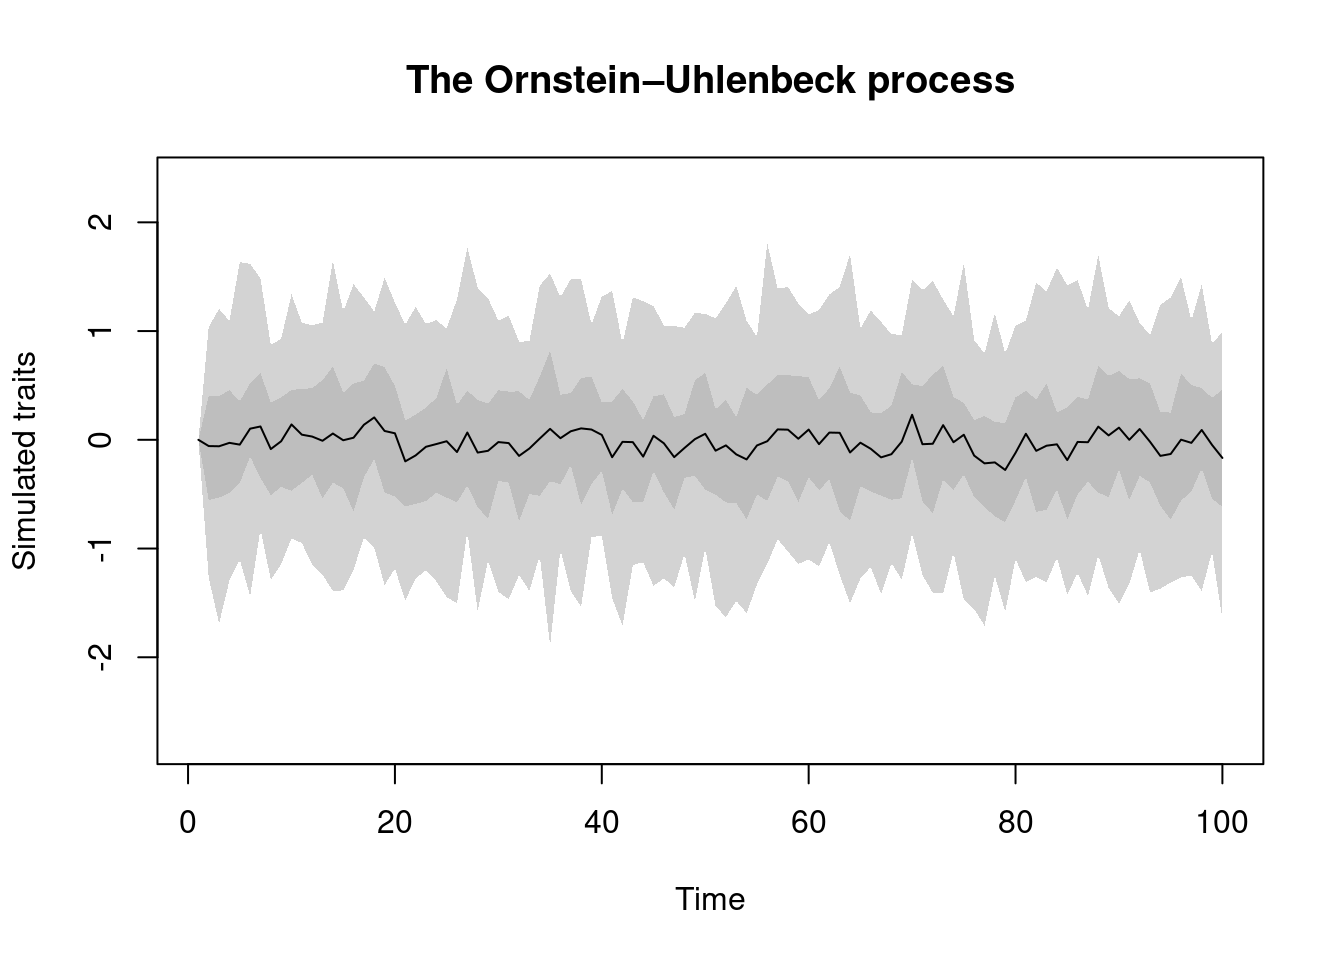
\includegraphics{dads_manual_files/figure-latex/unnamed-chunk-44-1.pdf}

\bibliography{../references.bib}

\end{document}
